%%
% 今時jarticleやjbook使ってる人いる?時代はjsarticleかjsbookだよ
% ついでに言うと、uplatexってのはplatexの上位互換、これを使わないなんて旧世代だよね
%
\documentclass[uplatex, report, a4j, 10pt]{jsbook}


%%
% パッケージ群
%
\usepackage{packages/miyazaki-u-paper}   % 宮崎大学工学部の卒論の基本(片山先生作)を、僕がちょっと書き換えちゃった(テヘッ
\usepackage{enumitem}           % enumerate?古い古い
\usepackage[dvipdfmx]{graphicx} % 当然dvipdfmなんて使ってないよね
\usepackage[dvipdfmx]{color}    % listingsを使うときにはこれも必須、dvipdfmxを変えちゃうとgraphicxのdvipdfmxも変わるよ
\usepackage{listings, packages/jlisting} % コードを埋め込むなら必須
\usepackage{txfonts}            % フォントといえばやっぱりtxfonts、今はnewtxってのもあるらしい
\usepackage{verbatim}           % コメントアウトしてくれる便利なプリアンブルが使える \begin{comment} ... \end{comment}
\usepackage{url}
% \usepackage{easy-todo}
\usepackage[hdivide={21mm, , 21mm}, vdivide={30mm, , 25mm}]{geometry} % スタイルを少し変えたくても\hoffset, \voffsetは使わないでね
\usepackage{multirow}
\usepackage{ascmac}

\renewcommand{\theenumi}{\arabic{enumi}.}
\renewcommand{\theenumii}{\alph{enumii}.}
\renewcommand{\theenumiii}{\roman{enumiii}.}

\renewcommand{\labelenumi}{\arabic{enumi}.}
\renewcommand{\labelenumii}{\alph{enumii}.}
\renewcommand{\labelenumiii}{\roman{enumiii}.}


% \usepackage{latexsym}
% \usepackage{bmpsize}
% \usepackage{comment}

% \def\Underline{\setbox0\hbox\bgroup\let\\\endUnderline}
% \def\endUnderline{\vphantom{y}\egroup\smash{\underline{\box0}}\\}

\newcommand{\ttt}[1]{\texttt{#1}}

%%
% miyazaki-u-paper.sty用設定値
%
\degree{m} % Graduateのg or Masterのm
\figurenumbering{f} % 図目次を付ける場合はt (真) を持つ真偽値を引数に取る関数
\tablenumbering{f} % 表目次を付ける場合はt (真) を持つ真偽値を引数に取る関数
\title{自然言語仕様書を入力とした\\機械学習によるVDM++仕様書\\自動生成ツールVGMLの開発}
\author{菅 健将}
\nendo{2} % 年度
\advisor{片山 徹郎 教授} % 修論では無視する
\major{工学専攻 機械・情報系コース 情報システム工学分野}


\begin{document}
\maketitle

%
% 概要
% 
\preface{概要}
ここに概要を書く。


%
% 本文
% 
\input{chapters/10-introduction.tex}
\chapter{研究の準備}
\label{cha:Preparation}

本章では、VGMLを開発するために必要となる前提知識を説明する。

\section{VDM++}
\label{sec:vdm}

形式手法の1つに、VDM(Vienna Development Method)がある\cite{}。
VDMは、1970年代にIBMのウィーン研究所にてPL/Iコンパイラの正しさを検証するために開発された形式手法である。
1996年には、形式仕様記述言語VDM-SLが標準となっている\cite{}。
VDM++は、VDM-SLを基にオブジェクト指向拡張した言語であり、現在VDMの中では主流である。

本研究では、VDM++仕様書を自動生成する。
VDM++は、VDMTools\cite{}やVDMJ\cite{}などの支援ツールが揃っており、他の形式手法に比べ仕様の検証がしやすい利点がある。
表\ref{table:vdm_block}に、VDM++の定義ブロックと、定義ブロックに対応する日本語での呼び方を示す。

\begin{table}[t]
    \begin{center}      
        \caption{VDM++の定義ブロックと定義ブロックに対応する日本語での呼び方}\label{table:vdm_block}
        \begin{tabular}{c|c}
        VDM++の定義ブロック  & 日本語での呼び方 \\ \hline \hline
        class & クラス \\ \hline
        types	 & 型定義 \\ \hline
        values  & 定数定義 \\ \hline
        instance variables & インスタンス変数定義 \\ \hline
        operations & 操作定義 \\ \hline 
        functions  & 関数定義 \\ \hline 
        \end{tabular}
    \end{center}
\end{table}

本研究では、表\ref{table:vdm_block}におけるVDM++の定義ブロックであるクラス、型定義、定数定義、インスタンス変数定義、操作定義に対応する。
各定義ブロックの詳細を、以下に示す。

\begin{itemize}
    \item クラス\\クラスは、プログラムにおけるクラスを表し、VDM++仕様書の構成単位である。オブジェクトはクラスのインスタンスである。
    \item 型定義\\プログラムにおけるデータ型を表す。ただし、本研究で定義の対象とする型は、realのみとする。
    \item 定数定義\\プログラムにおける定数を表す。
    \item インスタンス変数定義\\オブジェクトの中に保持される属性を表す。
    \item 操作定義\\オブジェクトの振る舞いを表すものの内、インスタンス変数を参照できる振る舞いを表す。
\end{itemize}

表\ref{table:vdm_syntax}に、本研究で対象としているVDM++の各定義ブロックの構文を示す。
各定義ブロックには、それぞれ対応する構文がある。また、構文は、VDM++における記述方法であり、複数の要素で構成する。
今回対象としている定義ブロックの構文の詳細を以下に示す。

\begin{itemize}
    \item class\\「class」の構文は「名前」の1つの要素を持つ。ここで、「名前」は定義するクラスの名前である。
    \item types\\「types」の構文は、「名前」の1つの要素を持つ。ここで、「名前」は定義する型の名前である。
    \item values\\「values」の構文は、「名前」と「値」の2つの要素を持つ。ここで、「名前」は定義する定数の名前、「値」は実数値である。
    \item instance variables\\「instance variables」の構文は、「名前」と「型」の2つの要素を持つ。ここで、「名前」は定義するインスタンス変数の名前、「型」は定義する型の名前である。
    \item operations\\「operations」の構文は、「名前」の1つの要素を持つ。ここで、「名前」は定義するメソッドの名前を表す。
\end{itemize}

\begin{table}[t]
    \begin{center}      
        \caption{VDM++の各ブロックの構文}\label{table:vdm_syntax}
        \begin{tabular}{c|c}
        定義ブロック  & 構文 \\ \hline \hline
        class & 名前 \\ \hline
        types	 & public 名前 = real ;\\ \hline
        values  & 名前 = 値 ;\\ \hline
        instance variables & public 名前 : 型 ;\\ \hline
        operations & 名前 : () ==\textgreater real\\
                   & 名前()==\\
                   & return 0 ;\\ \hline 
        \end{tabular}
    \end{center}
\end{table}

\section{WordNet}
\label{sec:wordNet}
WordNetは、1980年代にプリンストン大学で開発された、名詞の同義語、上位概念、下位概念など、
英語の名詞同士の意味的な関係に基づいて作成された辞書である\cite{}。
WordNetを日本語に対応できるように拡張したものとして、日本語WordNetがある\cite{}。
日本語WordNetは、57,238個の概念と、93,834個の単語を持つ。

本研究では、VDM++におけるクラスおよびインスタンス変数の候補となる単語を、
自然言語仕様書から抽出する際に、日本語WordNetを使用する\cite{}。
具体的には、自然言語仕様書内の単語に対し、機械学習に必要なパラメータとして本研究で新たに定義する概念レベルを計算する際に日本語WordNetを用いる。
概念レベルの計算は、\ref{sec:wordNet}節で述べた日本語WordNetを用いて、解析対象である単語の同義語とその下位概念の関係を表す木構造を生成する。
単語の下位概念の関係を表す木構造の例を、図\ref{fig:tree_structure}に示す。図\ref{fig:tree_structure}は、"りんご"の文字列を入力した際の木構造の例である。
日本語WordNetは、日本語での入力に対応しているが、出力する概念を表す単語は英語表記であるため、木構造を構成する単語も英語表記となる。
図\ref{fig:tree_structure}の木構造の場合、りんごの概念を持つ同義語を最上位のノードとし、その下位概念である単語を子ノードとして表現する。

\begin{figure}[t]
    \begin{center}
        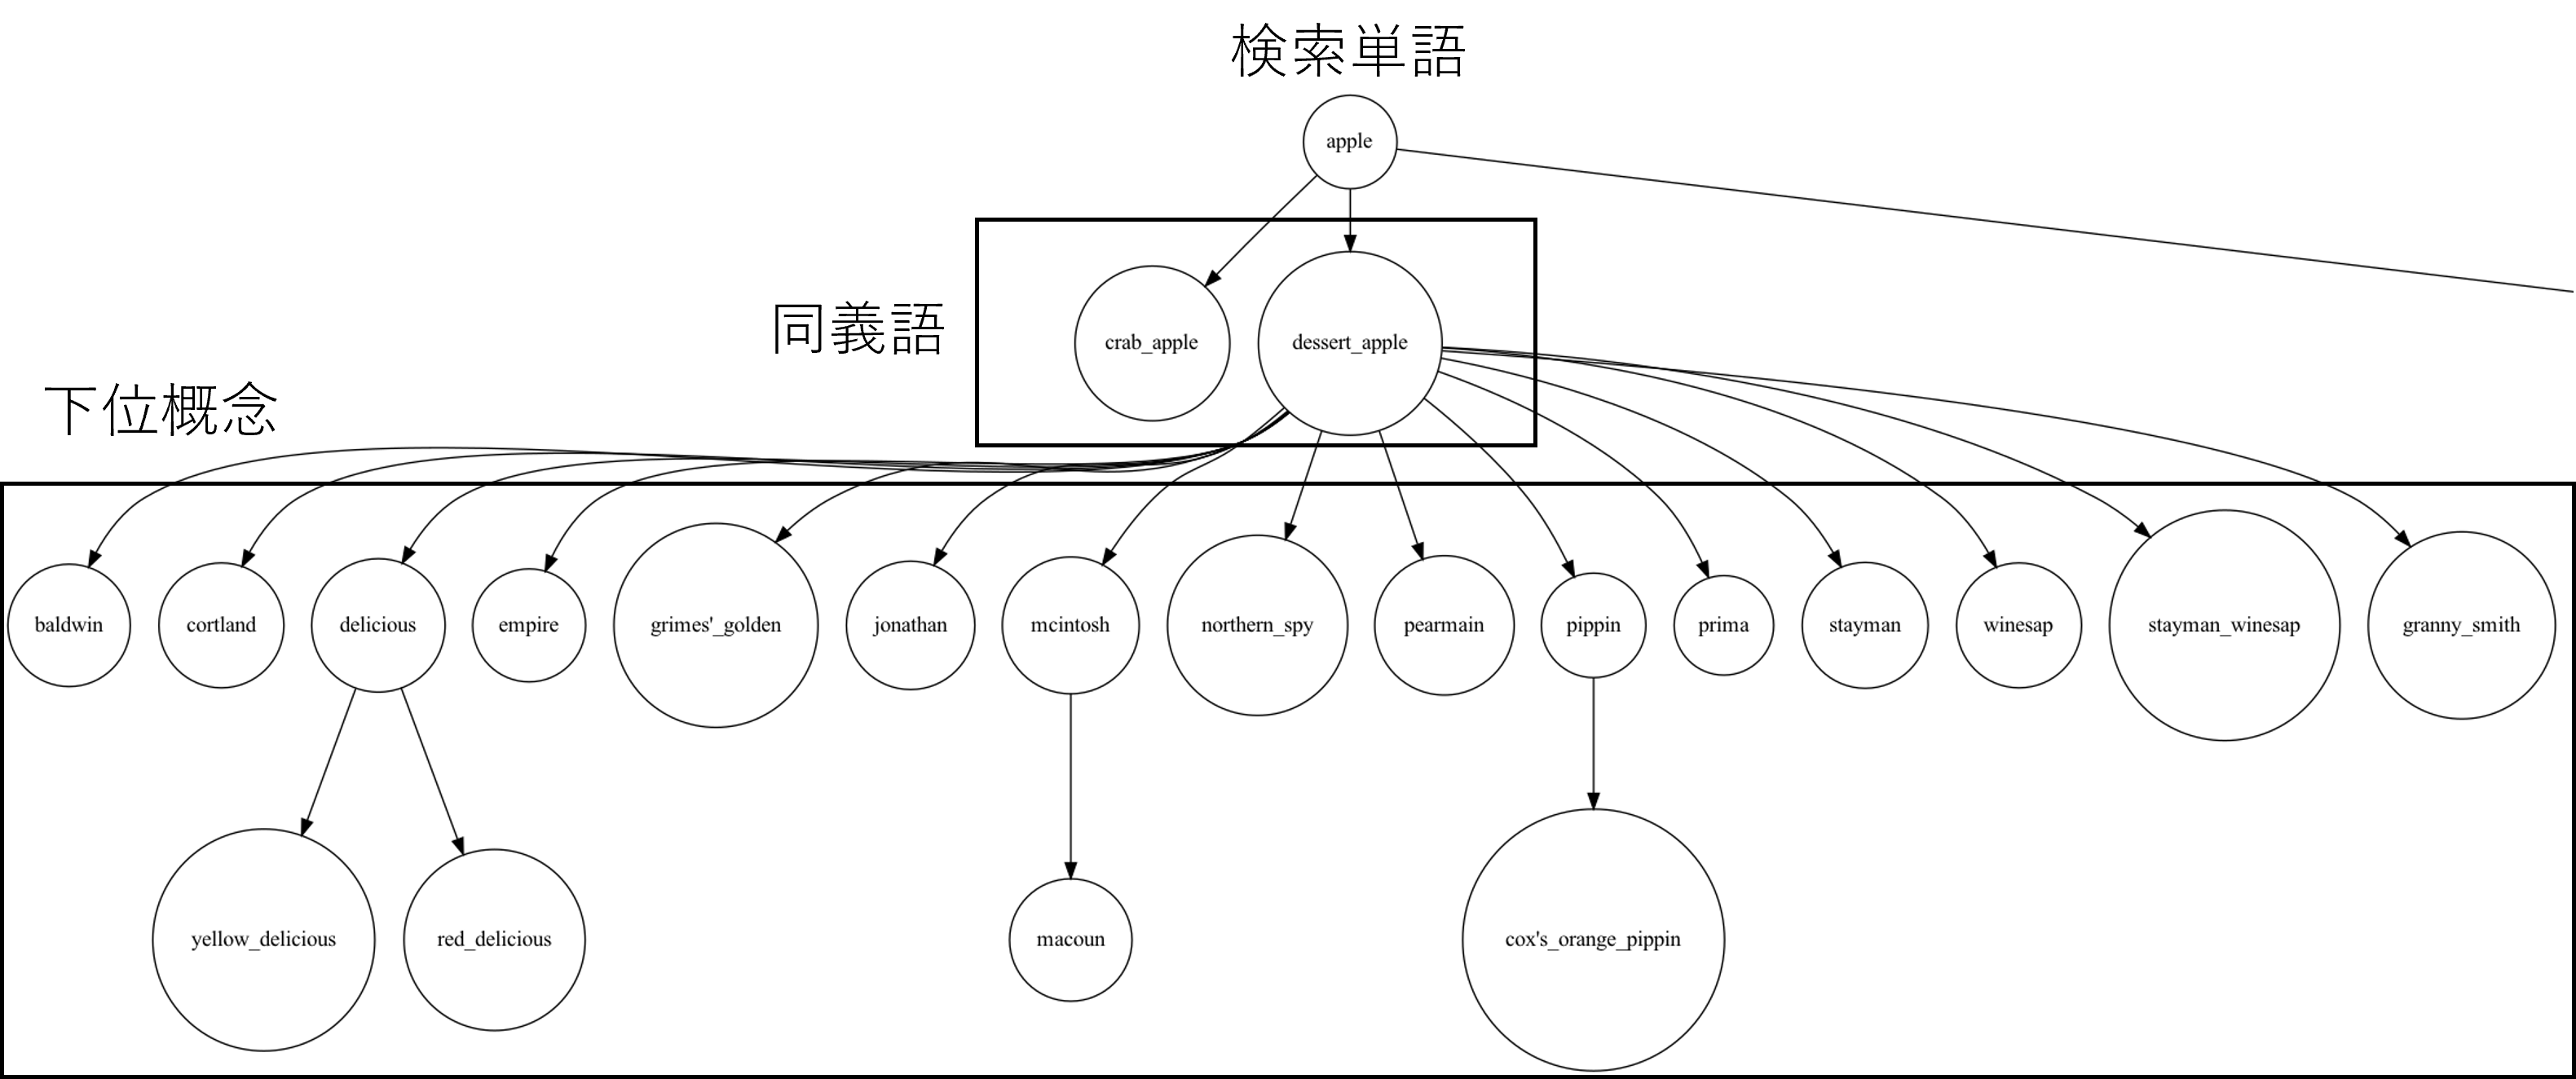
\includegraphics[width=1.0\columnwidth]{image/tree_structure.png}
        \caption{``りんご''を入力した際の下位概念の関係を表す木構造の例}
        \label{fig:tree_structure}
    \end{center}
\end{figure}

\section{Mecab}
\label{sec:mecab}
日本語の形態素解析を目的として、C++言語で開発されたオープンソースソフトウェアにMeCabがある\cite{}。
MeCabを用いることによって、日本語で記述された文書の分かち書きや、単語の品詞を取得できる。

本研究では、自然言語仕様書から単語とその単語の品詞を取得するために、MeCabを用いて自然言語仕様書内の文を形態素解析する。

\section{TfidfVectorizer}
\label{sec:tfidf}
文書内の単語の特徴量を得る手法の1つとして、TF-IDF法(Term Frequency Inverse Document Frequency Method)
がある\cite{}。TF-IDF法は、特定の文書にだけ頻繁に現れる単語に、大きな重みを与えるTF法と、コーパス中の多数の文書に現れる単語に、あまり重みを与えないIDF法の、
2つの手法によって計算する手法である。この手法によって計算された値は、TF-IDF値と呼ばれる。
TF-IDFを計算するためのオープンソースライブラリの1つに、scikit-learnがある。
scikit-learnは、機械学習ライブラリを多様に用意しており、その中のTfidfVectorizerクラスを利用することで、TF-IDF値を計算できる\cite{}。

本研究では、TfidfVectorizerを用いて、自然言語仕様書内の単語に対し、機械学習に必要なパラメータとしてTF-IDF値を計算する。

\section{ロジスティック回帰}
\label{sec:logistic}
ロジスティック回帰は、様々な種類の問題をモデル化することを目的として使用される統計手法の1つである。
統計学において、ある結果が起こる確率を予測する手段としてよく知られている手法であり、特に分類タスクで広く使われる。

式\ref{eq:logistic}に、ロジスティック回帰を示す。

\begin{equation}\label{eq:logistic}
    y = \log{(\frac{1}{1-p})}= \beta_{0}+ \beta_{1}\alpha_{1}+\beta_{2}\alpha_{2}+...+\beta_{x}\alpha_{x}
\end{equation}
$y$は、目的変数である確率$p$を説明変数$\alpha_{x}$と線形な関係になるように変換した値である。
$\beta_{0}$は、定数であり、$\beta_{1}~\beta_{x}$は、偏回帰変数である。

判定結果が2つのみの予測に使用できるロジスティック回帰を作成するために、2値ロジスティック回帰がある\cite{two_logistic}。
2値ロジスティック回帰は、$y$の値が0.5以上の場合は確率を1.0とみなし、0.5未満の場合は確率を0.0とみなすことによって、目的変数を判定する手法である。

式\ref{ep:two_logistic}に、2値ロジスティック回帰を示す。
式\ref{eq:logistic}をロジット変換で0から1に変換したものである。
\begin{equation}\label{eq:two_logistic}
    p = \frac{1}{1+exp[- (\beta_{0}+ \beta_{1}\alpha_{1}+\beta_{2}\alpha_{2}+...+\beta_{x}\alpha_{x})]}
\end{equation}

判定結果が3つ以上の予測に使用できるロジスティック回帰を作成するために、多項ロジスティック回帰がある\cite{multinomial_logistic}。
多項ロジスティック回帰モデルでは、3つ以上ある目的変数の値のうち、1つを基準としたロジスティック回帰モデルを、
目的変数の数より1つ少ない数だけ作成する。
目的変数がA,B,Cの3種類であり、Aを基準として考えた場合、式\ref{}と式\ref{}の2つの回帰モデルを作成する。

\begin{equation}\label{eq:logistic}
    y = \log{(\frac{B}{A})}= \beta_{0}+ \beta_{1}\alpha_{1}+\beta_{2}\alpha_{2}+...+\beta_{x}\alpha_{x}
\end{equation}

\begin{equation}\label{eq:logistic}
    y = \log{(\frac{C}{A})}= \beta_{0}+ \beta_{1}\alpha_{1}+\beta_{2}\alpha_{2}+...+\beta_{x}\alpha_{x}
\end{equation}



既存ツールは、単語をVDM++仕様書に必要であるか否かの判定を行うために、機械学習のモデルとして、2値ロジスティック回帰モデルを用いる。
   
2値ロジスティック回帰のアルゴリズムを用いるモデルは「教師あり学習」手法である。
このため、モデルをトレーニングするための結果をあらかじめ含んだデータセットを用意する必要があり、
データをロジスティック関数にフィッティングすることで事象の発生確率を予測する。

本研究では、単語に対してVDM++仕様書に必要な単語であるか否かの判定を行うために、機械学習のモデルとし
\chapter{既存手法}\label{cha:Function}

本章では、既存手法について説明する。
既存手法は、自然言語仕様書を入力として、型定義と定数定義を記述したVDM++仕様書を出力する。

既存手法の構造を、図\ref{fig:exis_structure}に示す。既存手法は、以下の4つの処理部で構成する。

\begin{figure}[tp]
    \begin{center}
        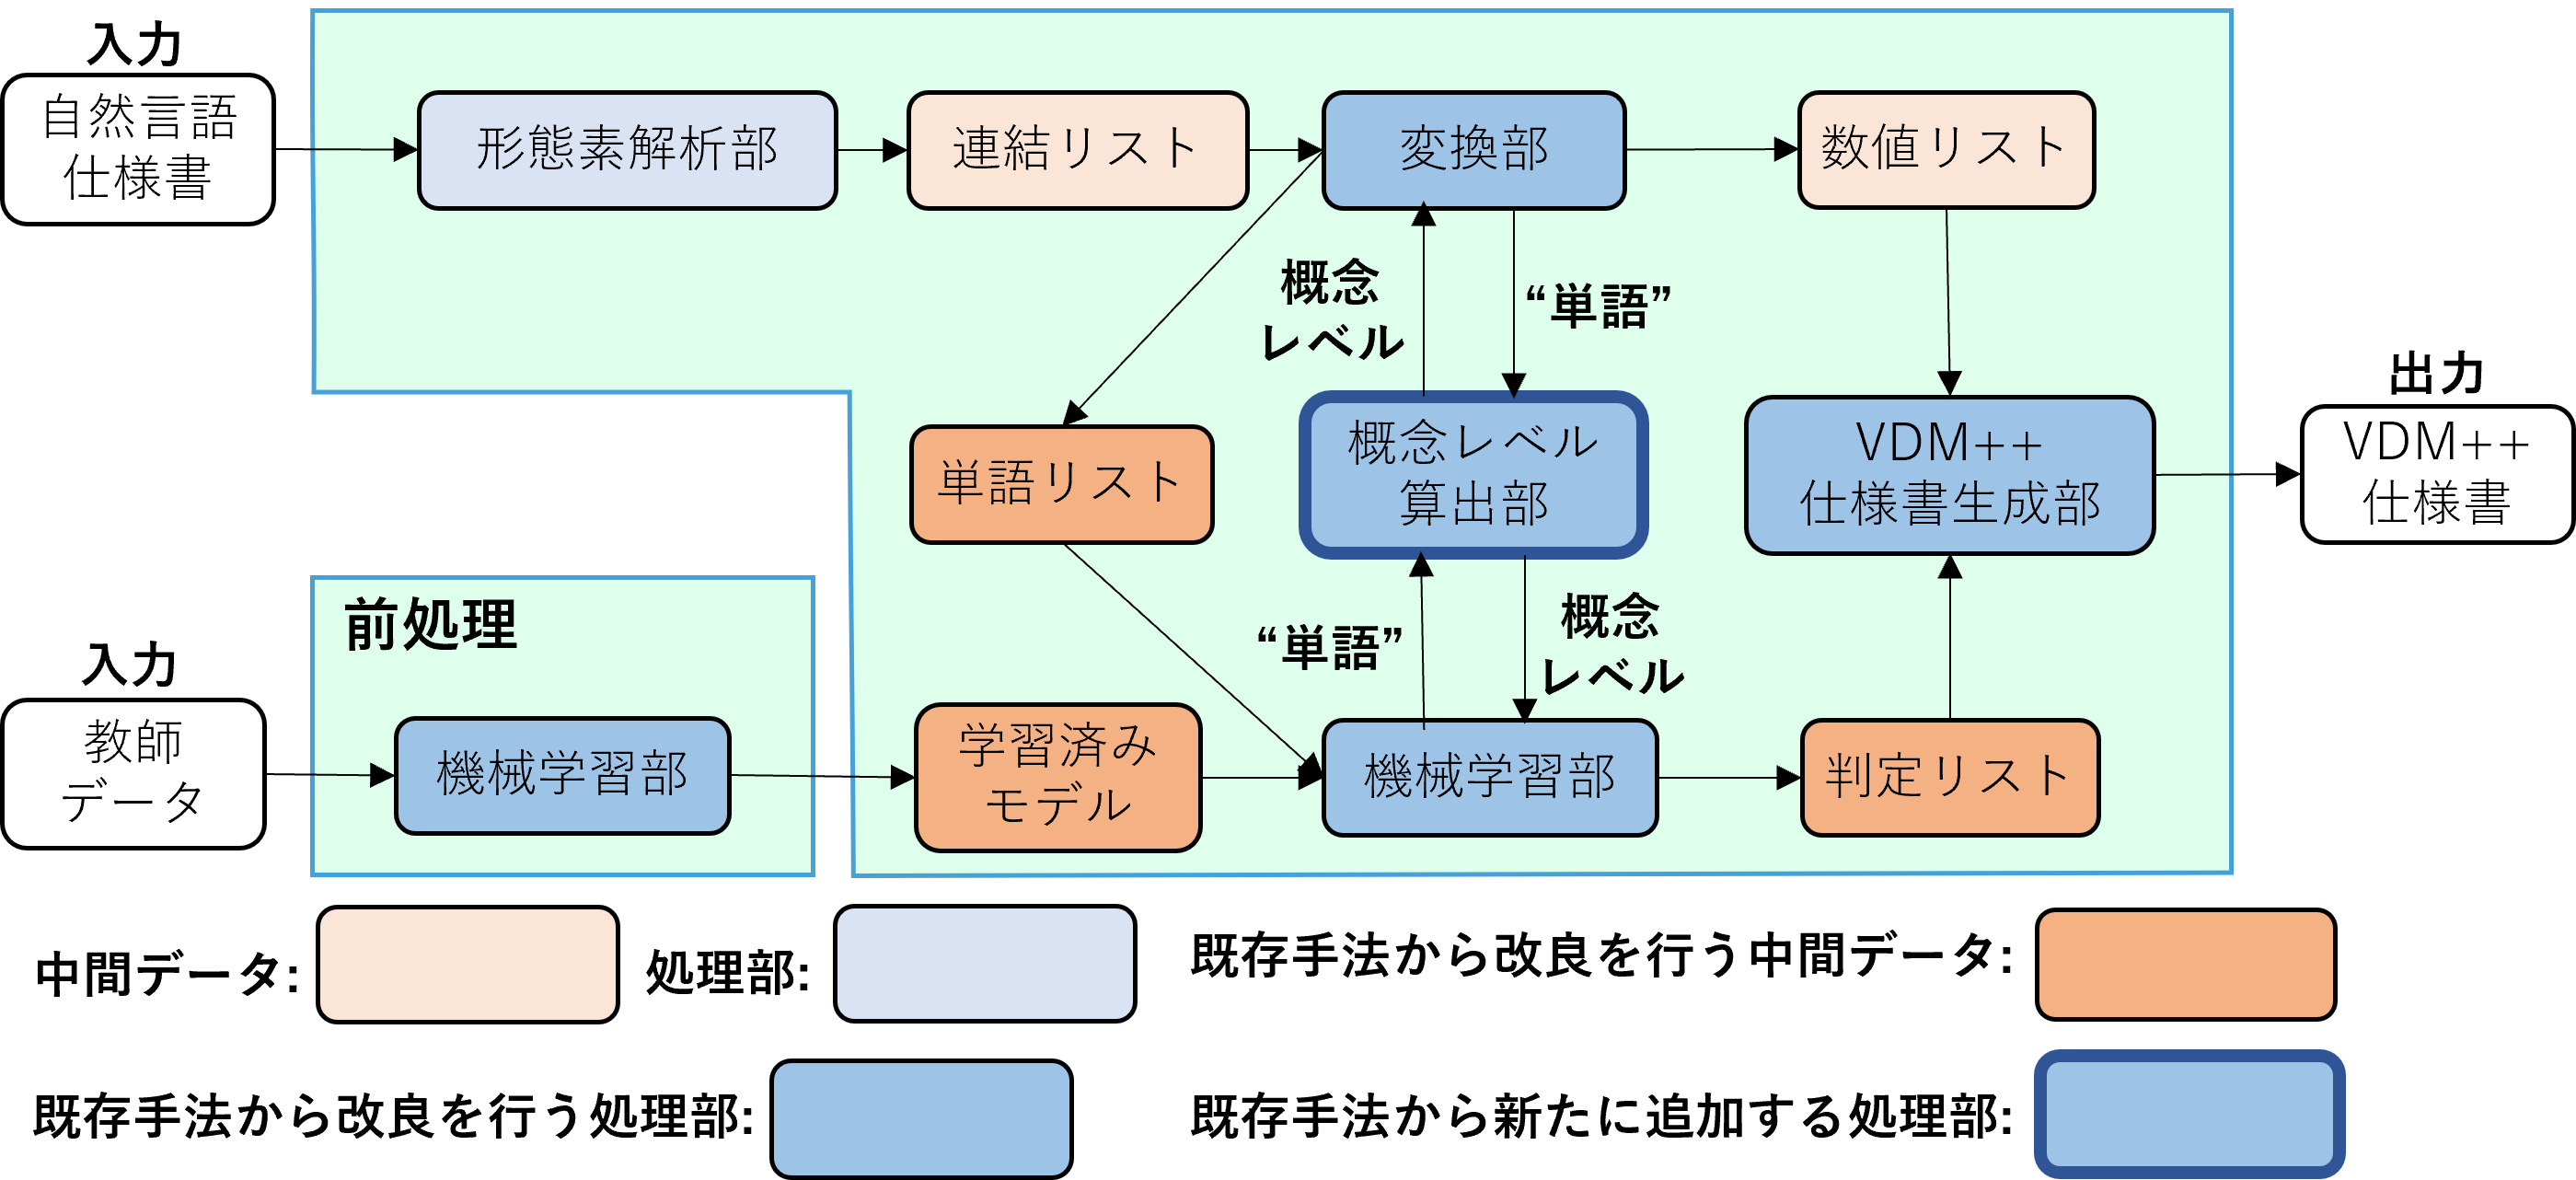
\includegraphics[width=1.0\columnwidth]{image/vgml_structure.png}
        \caption{既存手法の構造}
        \label{fig:exis_structure}
    \end{center}
\end{figure}

\begin{itemize}
    \item 形態素解析部
    \item 変換部
    \item 機械学習部
    \item VDM++仕様書生成部
\end{itemize}

以降、4つの処理部について詳細を説明する。

\section{形態素解析部}
既存手法における形態素解析部は、wordまたはpdfで記述された自然言語仕様書を入力として、連結リストを出力する。
既存手法が入力とする自然言語仕様書の例を図\ref{fig:exis_spec_example}に、既存手法における形態素解析部の構造を、図\ref{fig:exis_mor_structure}に示す。
既存手法における形態素解析部の処理の流れを、以下に示す。

\begin{enumerate}
    \item テキスト抽出処理において、自然言語仕様書を入力とし、自然言語仕様書内のテキストを抽出する。さらに、抽出したテキストを格納したテキストリストを生成する。図\ref{fig:exis_spec_example}に示す仕様書を入力として、既存手法のテキスト抽出処理が生成するテキストリストを、図\ref{fig:exis_text_list}に示す。
    \label{text_list}
    \item 分かち書き処理において、\ref{text_list}で生成したテキストリストを入力とし、テキストリスト内のテキストを文ごとに分ける。さらに、文を\ref{}節で述べたMecabを用いて分かち書きし、分かち書きした文を格納した分かち書きリストを生成する。図\ref{fig:text_list}に示すテキストリストを入力として、既存手法の分かち書き処理が生成する分かち書きリストを、図\ref{fig:exis_wakati_list}に示す。
    \label{wakati_list}
    \item 単語連結処理において、\ref{wakati_list}で生成した分かち書きリストを入力とし、分かち書きリスト内の助詞、助動詞、接続詞、副詞の品詞である単語を除く。さらに、分かち書きリスト内の文の連続する2つ以上の名詞と動詞を連結する。最後に、名詞と動詞を連結した文を格納した連結リストを生成する。図\ref{fig:wakati_list}に示す分かち書きリストを入力として、既存手法の単語連結処理が生成する連結リストを、図\ref{fig:exis_connect_list}に示す。
\end{enumerate}

\begin{figure}[tp]
    \begin{center}
        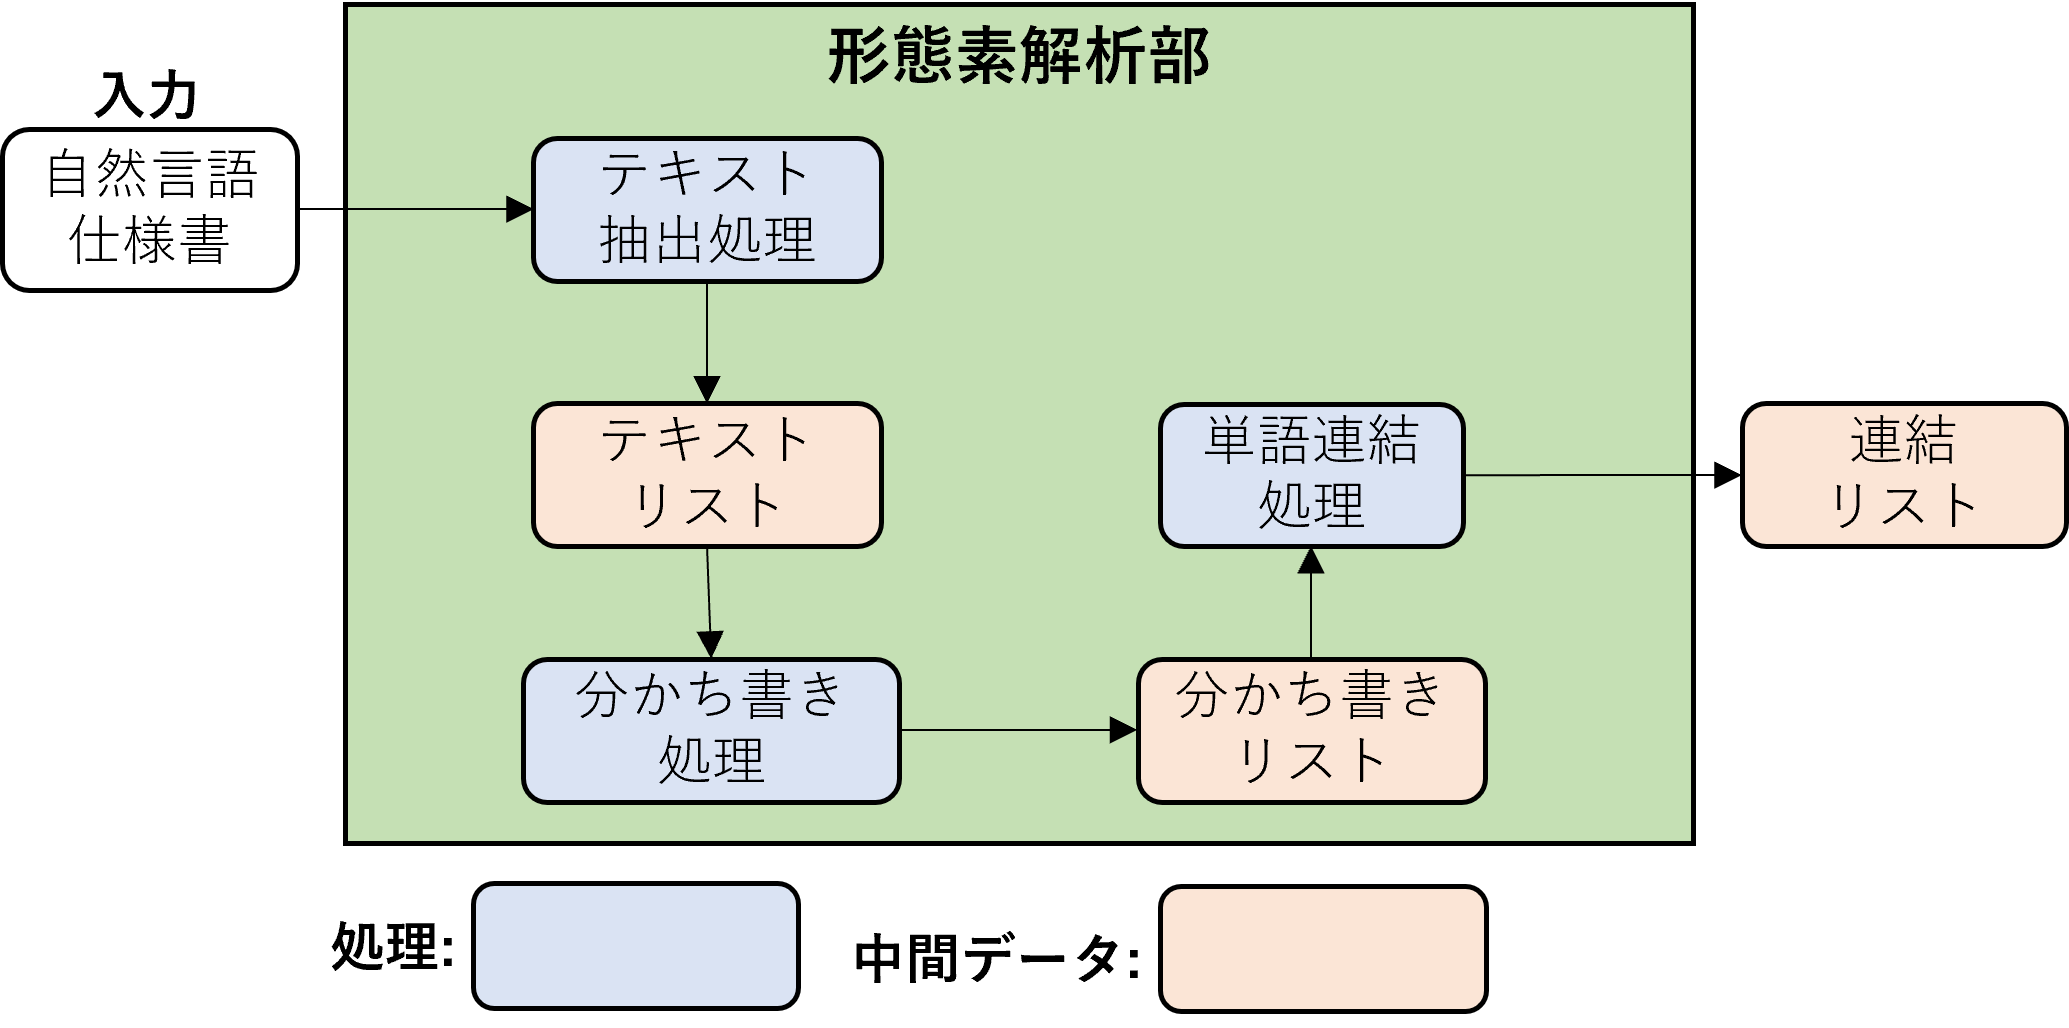
\includegraphics[width=1.0\columnwidth]{image/exis_mor_structure.png}
        \caption{既存手法における形態素解析部の構造}
        \label{fig:exis_mor_structure}
    \end{center}
\end{figure}

\begin{figure}[tp]
    \begin{center}
        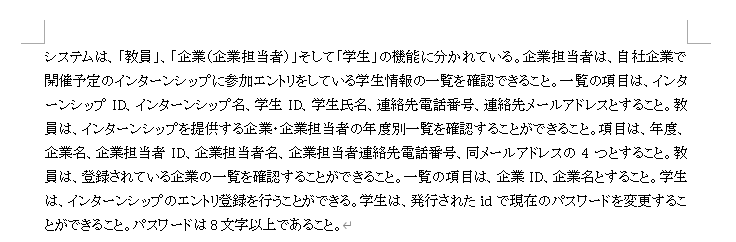
\includegraphics[width=1.0\columnwidth]{image/exis_spec_example.png}
        \caption{入力とする自然言語仕様書の例}
        \label{fig:exis_spec_example}
    \end{center}
\end{figure}

\begin{figure}[tp]
    \begin{center}
        
\includegraphics[width=1.0\columnwidth]{image/exis_text_list.png}
        \caption{既存手法のテキスト抽出処理が生成するテキストリスト}
        \label{fig:exis_test_list}
    \end{center}
\end{figure}

\begin{figure}[tp]
    \begin{center}
        
\includegraphics[width=1.0\columnwidth]{image/exis_wakati_list.png}
        \caption{既存手法の分かち書き処理が生成する分かち書きリスト}
        \label{fig:exis_wakati_list}
    \end{center}
\end{figure}

\begin{figure}[tp]
    \begin{center}
        
\includegraphics[width=1.0\columnwidth]{image/exis_connect_list.png}
        \caption{既存手法の形態素解析部が生成する連結リスト}
        \label{fig:exis_connect_list}
    \end{center}
\end{figure}

\section{変換部}
\label{sec:exis_transfer}
既存手法における変換部は、図\ref{fig:exis_connect_list}に示す連結リストを入力として、単語リストを生成する。
既存手法における変換部の構造を、図\ref{fig:exis_transfer_structure}に示す。
既存手法における変換部の処理の流れを、以下に示す。

\begin{enumerate}
    \item TF-IDF値生成処理において、図\ref{fig:exis_connect_list}に示す連結リストを入力とし、連結リスト内の単語に対し\ref{}で述べたTF-IDF値を計算する。さらに、連結リスト内の単語を全て格納した単語配列と、単語とTF-IDF値のセットを格納した列数2の一時ファイルを生成する。
    \label{tf_list}
    \item 出現回数生成処理において、\ref{tf_list}で生成した単語配列と列数2の一時ファイルを入力とし、単語配列の各単語の出現回数を計算する。さらに、列数2の一時ファイルに各単語の出現回数を追加することによって列数3の一時ファイルを生成する。
    \label{appear_list}
    \item 優先値生成処理において、\ref{appear_list}で生成した列数3の一時ファイルを入力とし、各単語の文字数とその文字の種類によって重みづけをした値(優先値)を計算する。さらに、列数3の一時ファイルに各単語の優先値を追加することによって列数4の一時ファイルを生成する。文字の種類によって重みづけをした値を表\ref{}に、優先値の計算式を式\ref{}に示す。
    \label{prior_list}
    \item 連結回数生成処理において、図\ref{fig:exis_connect_list}に示す連結リストと\ref{prior_list}で生成した列数4の一時ファイルを入力とし、各単語が他の単語に連結している回数を計算する。さらに、列数4の一時ファイルに各単語の連結回数を追加することによって単語リストを生成する。
    \label{exis_word_list}
    \item 数値抽出処理において、図\ref{fig:exis_connect_list}に示す連結リストと\ref{exis_word_list}で生成した単語リストを入力とし、各単語が同じ文中にその単語の数を表す数値があるかを探索する。さらに、単語、数値、TF-IDF値のセットを格納した数値リストを生成する。
\end{enumerate}

図\ref{fig:exis_connect_list}に示す連結リストを入力として、既存手法の変換部が生成する単語リストの一部を図\ref{fig:exis_connect_list}に、数値リストを図\ref{fig:exis_suti_list}示す。

\begin{figure}[tp]
    \begin{center}
        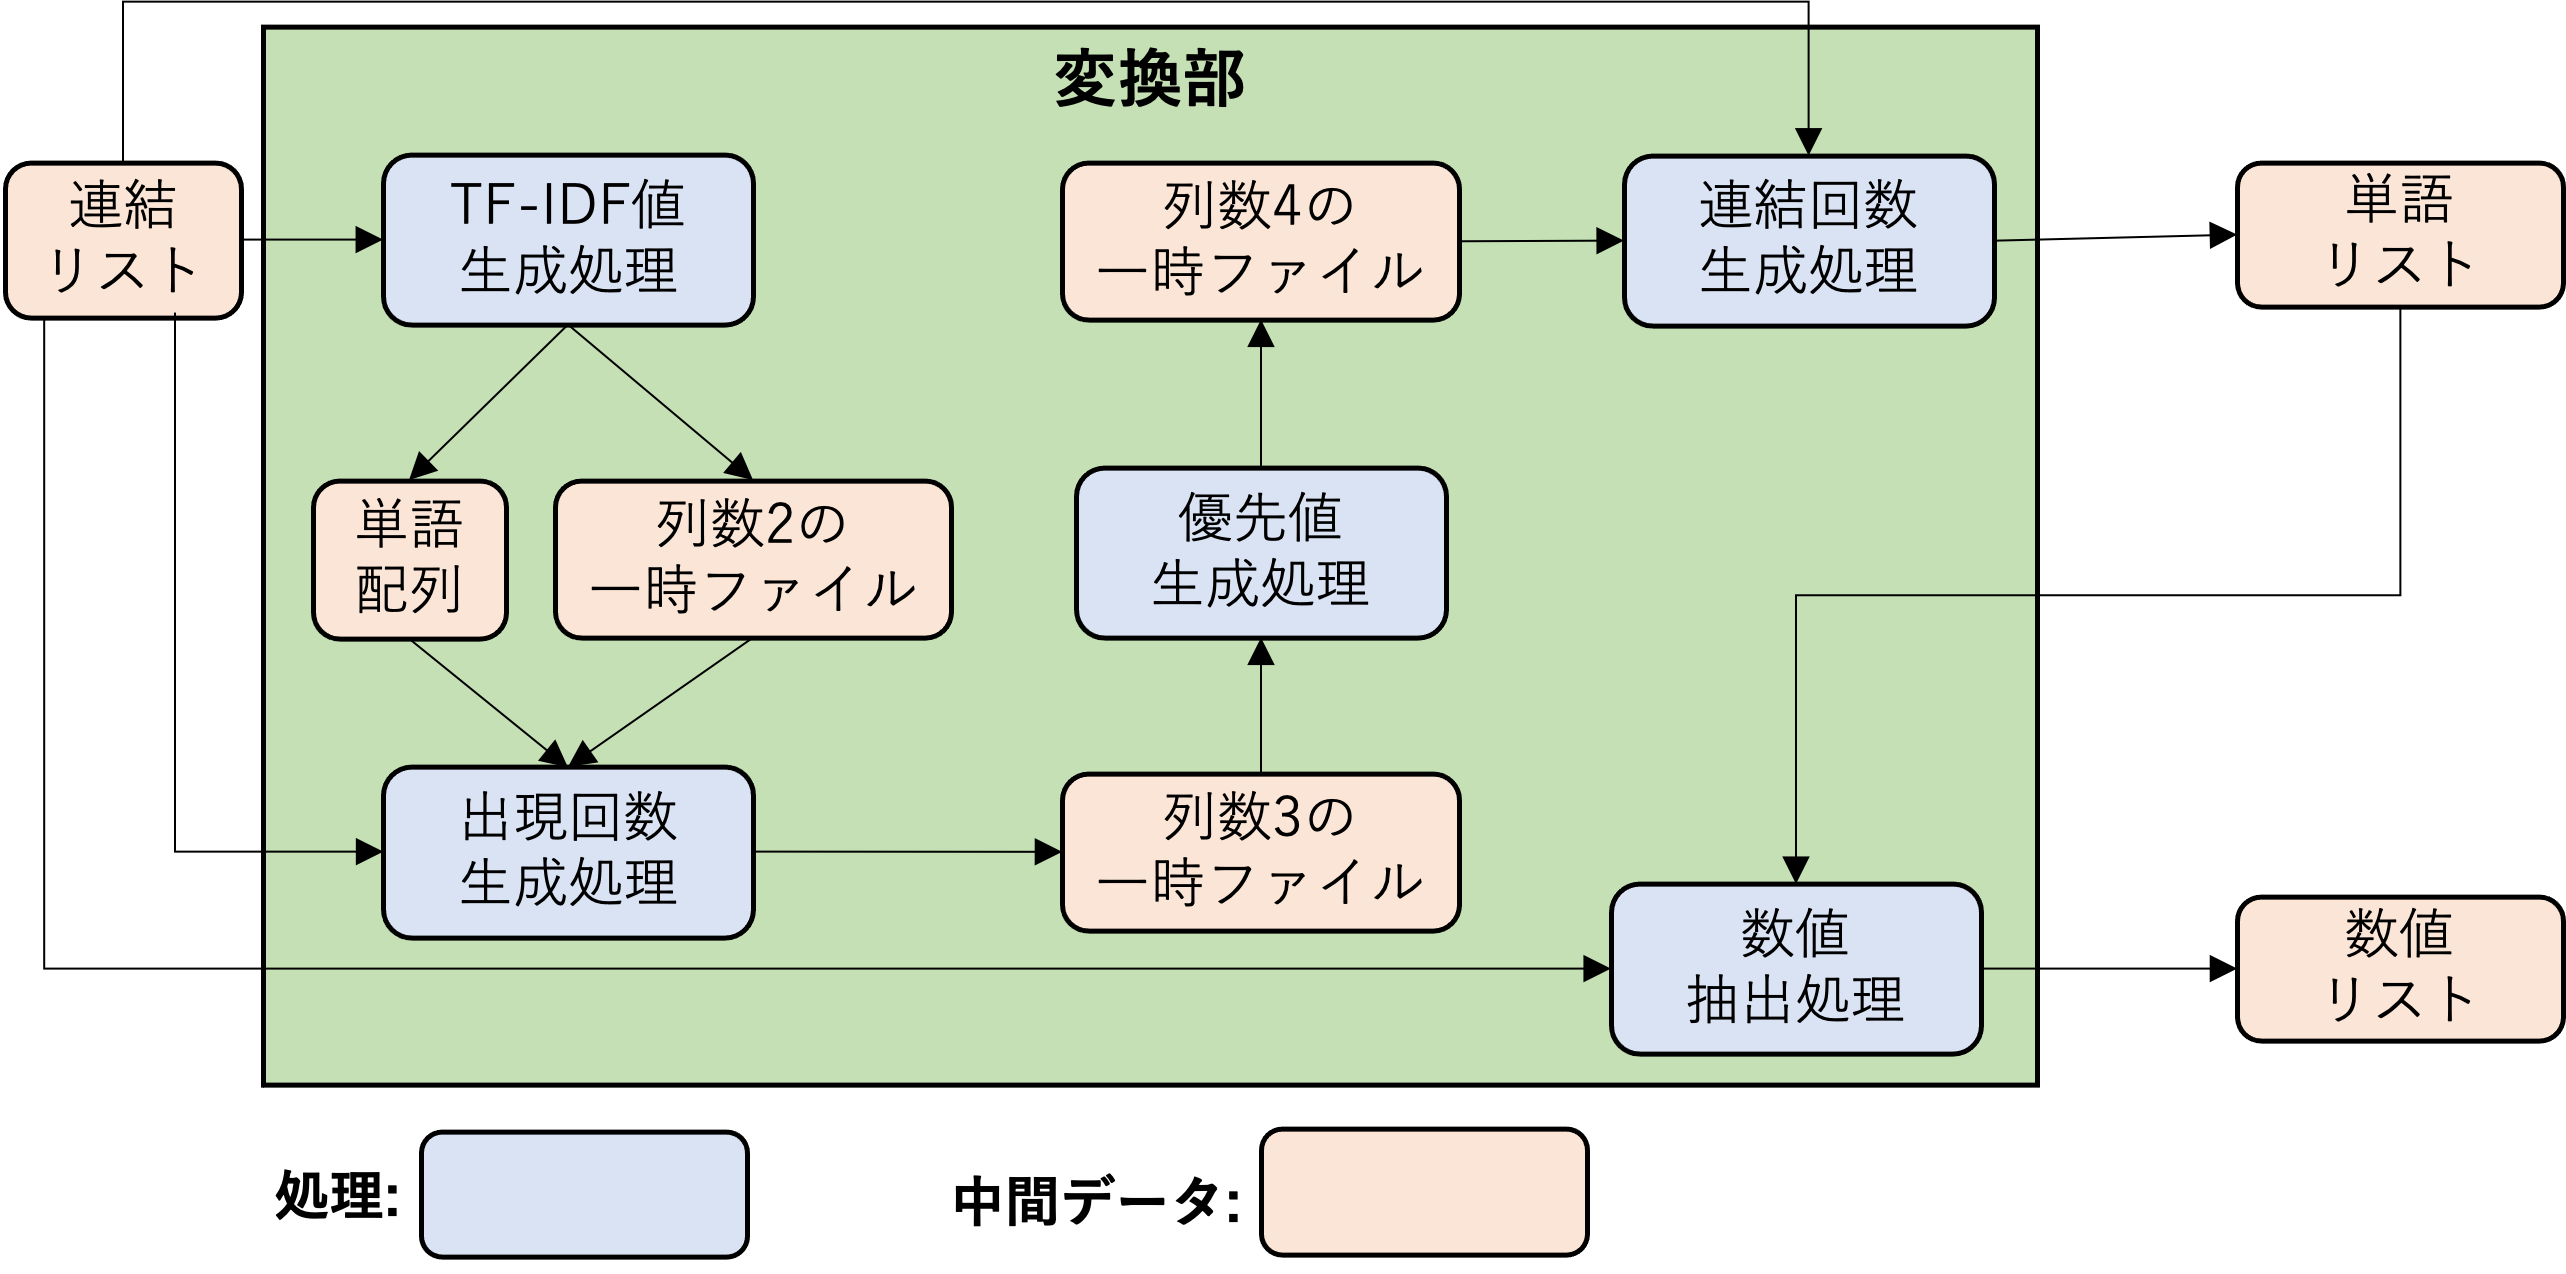
\includegraphics[width=1.0\columnwidth]{image/exis_transfer_structure.png}
        \caption{既存手法における変換部の構造}
        \label{fig:exis_transfer_structure}
    \end{center}
\end{figure}

\begin{figure}[tp]
    \begin{center}
        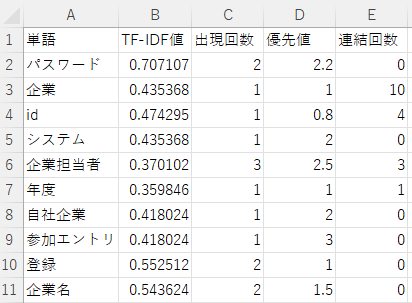
\includegraphics[width=300]{image/exis_word_list.png}
        \caption{既存手法の変換部が生成する単語リストの一部}
        \label{fig:exis_word_list}
    \end{center}
\end{figure}

\begin{figure}[tp]
    \begin{center}
        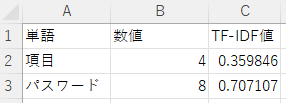
\includegraphics[width=180]{image/exis_suti_list.png}
        \caption{既存手法の変換部が生成する数値リスト}
        \label{fig:exis_suti_list}
    \end{center}
\end{figure}

\section{機械学習部}
\label{sec:exis_machine}
既存手法における機械学習部は、2つの役割を持つ。1つは、前処理として、教師データを入力とし、学習済みモデルを出力する。
もう一つは、単語リストと学習済みモデルを入力とし、判定リストを出力する。
既存手法における機械学習部の構造を、図\ref{fig:exis_machine_structure}に、既存手法の機械学習部が入力とする教師データの一部を、図\ref{fig:exis_teach}に示す。
また、学習済みモデルについては、「インターンシップ評定書・オンライン提出システム」によって生成した学習済みモデルを使用する。
「インターンシップ評定書・オンライン提出システム」は、宮崎大学工学部情報システム工学科の演習科目「プログラミング演習5」の課題として使用された自然言語仕様書である。
付録A.に、「インターンシップ評定書・オンライン提出システム」の自然言語仕様書を示す。
既存手法の機械学習部が入力する教師データは、図\ref{fig:exis_word_list}に示す単語リストの単語の次の列に判定結果の列を挿入したものである。判定結果は、0または1の値を人手により与える。
0は単語がVDM++仕様書に必要でないことを表し、1は単語がVDM++仕様書に必要であることを表す。

表\ref{table:exis_data_set}に既存手法における教師あり学習のデータセット数を示す。

\begin{table}[t]
    \begin{center}
      \caption{既存手法における教師データのデータセット数}
      \label{table:exis_data_set}
      \begin{tabular}{c|c}
        データ総数 & 157\\
        \hline
        \hline
        VDM++仕様書に必要であるデータ    & 71\\ \hline
        VDM++仕様書に必要でないデータ & 86\\ \hline
      \end{tabular}
    \end{center}
  \end{table}

既存手法における機械学習部の処理の流れを、以下に示す。

\begin{enumerate}
    \item 学習済みモデル生成処理において、図\ref{fig:exis_teach}に示す教師データを入力とし、\ref{}節で述べた二項ロジスティック回帰分析を用いて学習済みモデルを生成する。
    \label{exis_teach_model}
    \item 判定リスト生成処理において、\ref{exis_teach_model}で生成した学習済みモデルと図\ref{exis_word_list}に示す単語リストを入力とし、単語リスト内の単語がVDM++仕様書に必要である確率を計算する。さらに、確率が0.5未満である単語に0の判定結果を、確率が0.5以上の単語に1の判定結果を与える。最後に、単語リストに単語の判定結果と確率を追加することによって判定リストを生成する。
\end{enumerate}

図\ref{fig:exis_teach}に示す教師データを基に生成した学習済みモデルと、図\ref{fig:exis_word_list}に示す単語リストを入力として、既存手法の機械学習部が生成する判定リストの一部を図\ref{fig:exis_judge_list}に示す。

\begin{figure}[tp]
    \begin{center}
        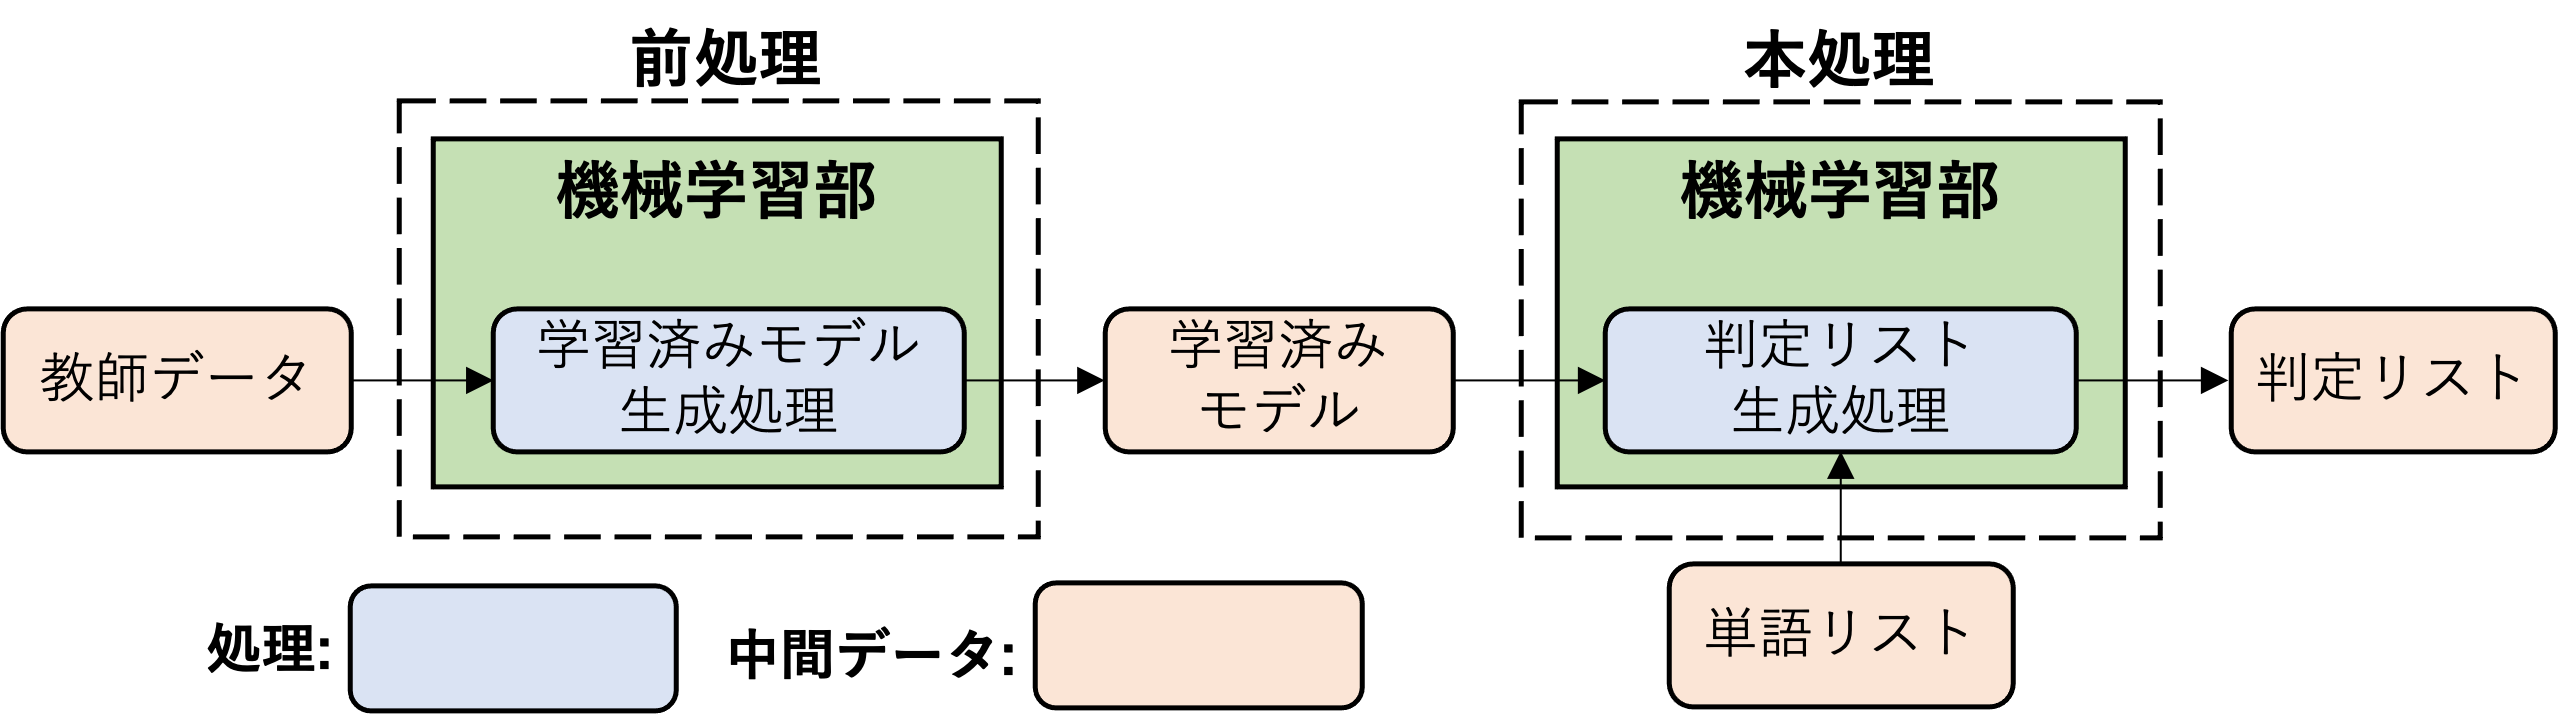
\includegraphics[width=1.0\columnwidth]{image/exis_machine_structure.png}
        \caption{既存手法における機械学習部の構造}
        \label{fig:exis_machine_structure}
    \end{center}
\end{figure}

\begin{figure}[tp]
    \begin{center}
        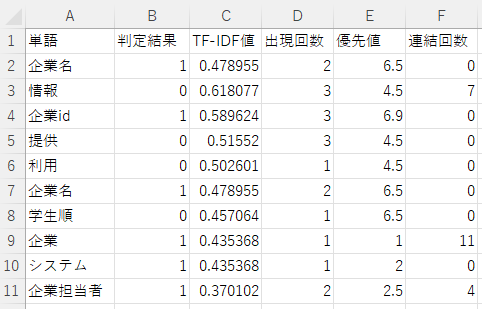
\includegraphics[width=300]{image/exis_teach.png}
        \caption{既存手法の機械学習部が入力とする教師データの一部}
        \label{fig:exis_teach}
    \end{center}
\end{figure}

\begin{figure}[tp]
    \begin{center}
        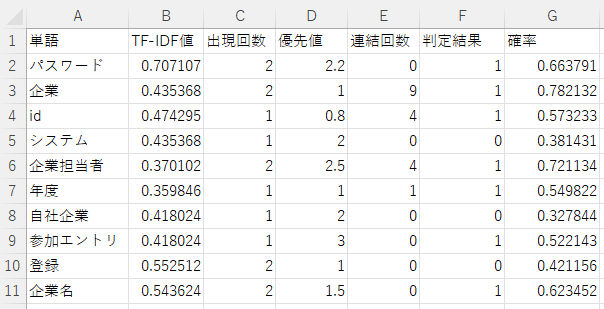
\includegraphics[width=300]{image/exis_judge_list.png}
        \caption{既存手法の機械学習部が生成する判定リストの一部}
        \label{fig:exis_judge_list}
    \end{center}
\end{figure}

\section{VDM++仕様書生成部}
既存手法におけるVDM++仕様書生成部は、図\ref{fig:exis_judge_list}に示す判定リストを入力として、VDM++仕様書を生成する。
既存手法におけるVDM++仕様書生成部の構造を、図\ref{fig:exis_generator_structure}に示す。
既存手法におけるVDM++仕様書生成部の処理の流れを、以下に示す。

\begin{enumerate}
    \item 型・定数定義生成処理において、図\ref{fig:exis_suti_list}に示す数値リストと、図\ref{fig:exis_judge_list}に示す判定リストを入力とし、識別子を挿入するための一時的なID「INDEX」と単語のセット、または「INDEX」、単語、数値のセットを格納した型・定数定義リストを生成する。図\ref{fig:exis_suti_list}と図\ref{fig:exis_judge_list}を入力として、既存手法の型・定数定義生成処理が生成する型・定数定義リストを、図\ref{fig:exis_katateisu_list}に示す。
    \label{katateisu}
    \item 識別子挿入処理において、\ref{katateisu}で生成した型・定数定義リスト内の一時的なID「INDEX」に、「types」または「values」を識別子として挿入する。さらに、識別子と単語のセット、または識別子、単語、数値のセットを格納した型・定数定義識別子リストを生成する。図\ref{fig:exis_katateisu_list}に示す型・定数定義リストを入力として、既存手法の識別子挿入処理が生成する型・定数定義識別子リストを、図\ref{fig:exis_katateisu_id_list}に示す。
    \label{sikibetu}
    \item VDM++仕様書生成部において、表\ref{table:vdm_syntax}の構文に従って、\ref{sikibetu}で生成した型・定数定義識別子リスト内の単語をVDM++仕様書の構文の「名前」に、数値をVDM++仕様書の構文の「値」に挿入する。さらに、構文に沿って単語と数値を挿入した後の文字列を、ファイルに記述することによってVDM++仕様書を生成する。図\ref{fig:exis_katateisu_id_list}に示す型・定数定義識別子リストを入力として、既存手法のVDM++仕様書生成処理が生成するVDM++仕様書を、図\ref{fig:exis_vdm}に示す。
\end{enumerate}

\begin{figure}[tp]
    \begin{center}
        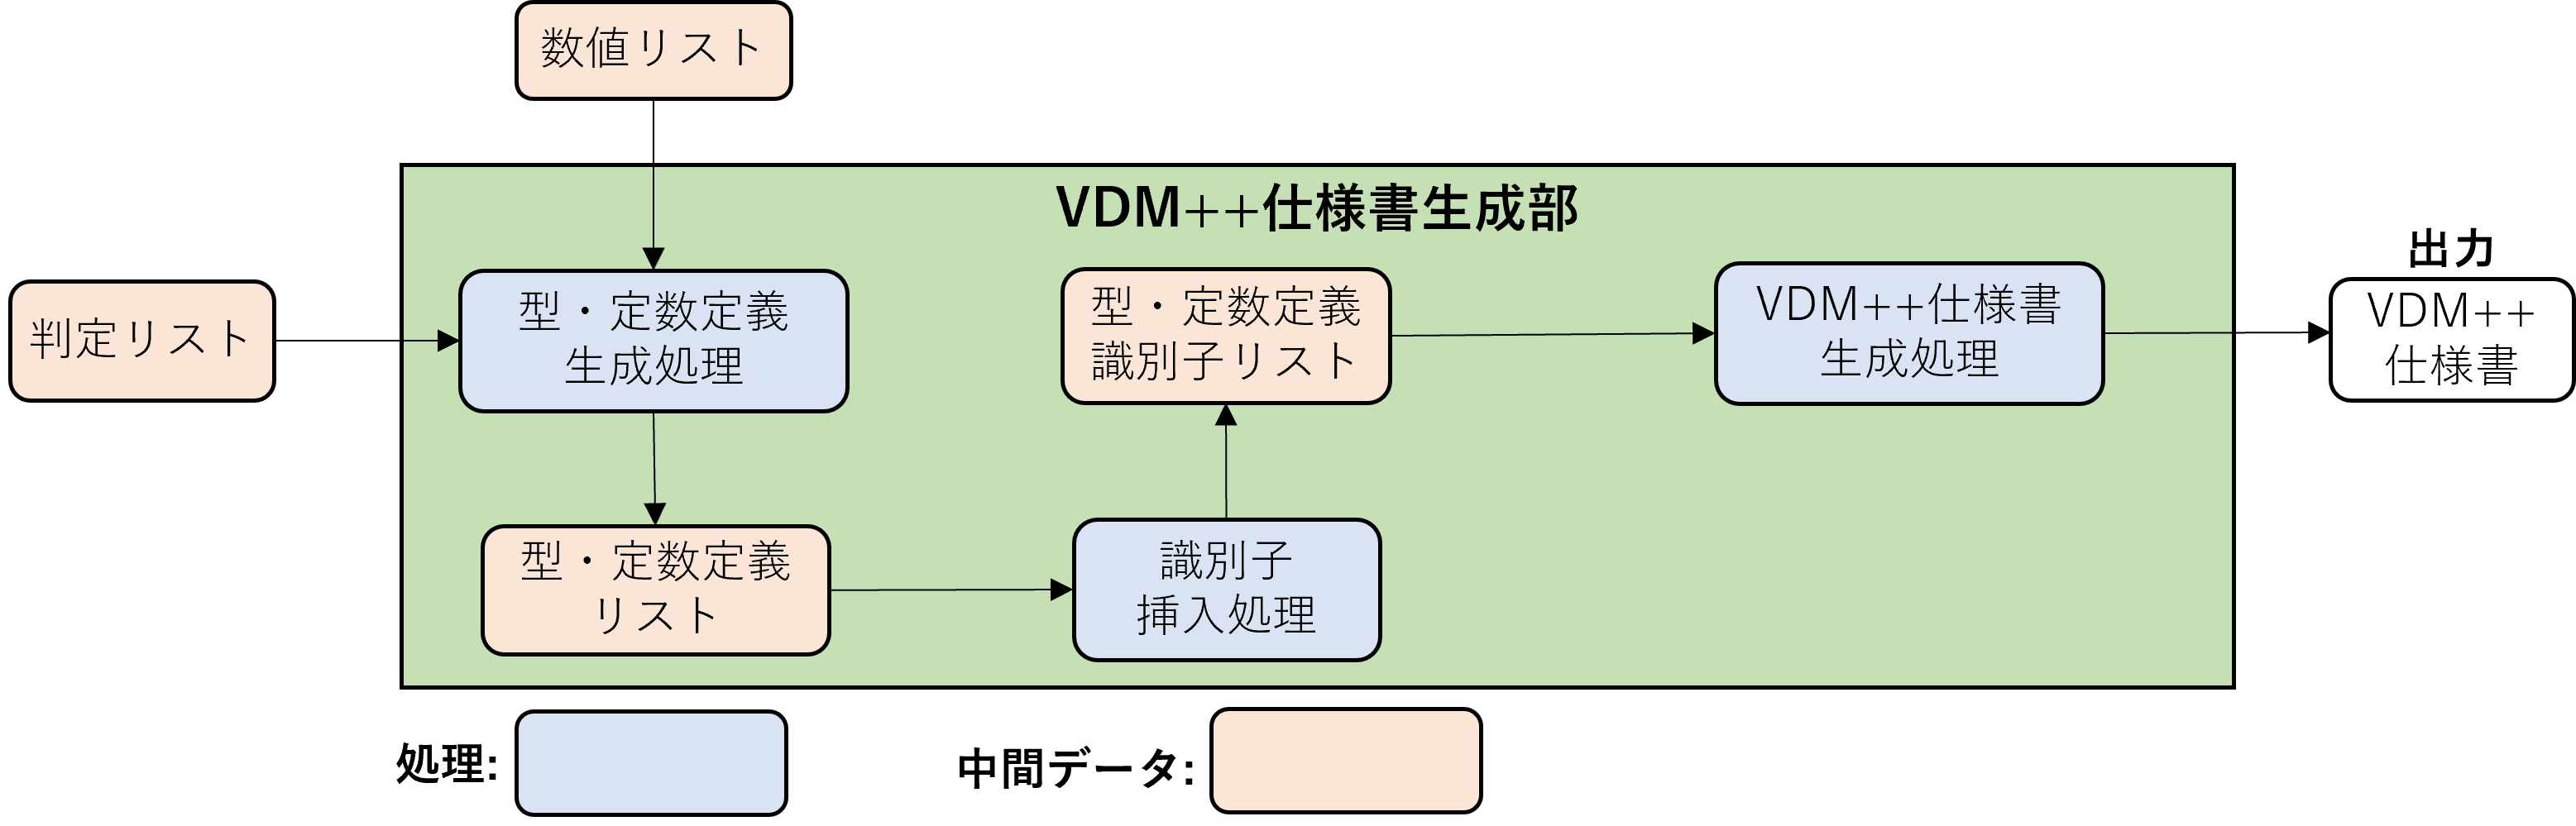
\includegraphics[width=1.0\columnwidth]{image/exis_generator_structure.png}
        \caption{既存手法におけるVDM++仕様書生成部の構造}
        \label{fig:exis_generator_structure}
    \end{center}
\end{figure}

\begin{figure}[tp]
    \begin{center}
        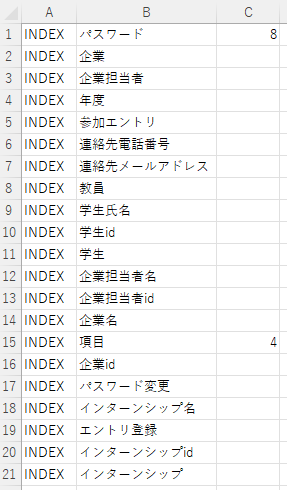
\includegraphics[width=300]{image/exis_katateisu_list.png}
        \caption{既存手法の型・定数定義生成処理が生成する型・定数定義リスト}
        \label{fig:exis_katateisu_list}
    \end{center}
\end{figure}

\begin{figure}[tp]
    \begin{center}
        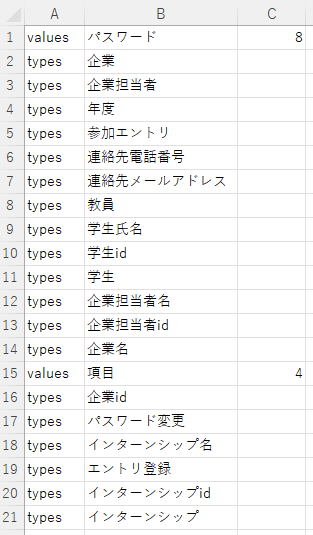
\includegraphics[width=300]{image/exis_katateisu_id_list.PNG}
        \caption{既存手法の識別子挿入処理が生成する型・定数定義識別子リスト}
        \label{fig:exis_katateisu_id_list}
    \end{center}
\end{figure}


\begin{figure}[tp]
    \begin{center}
        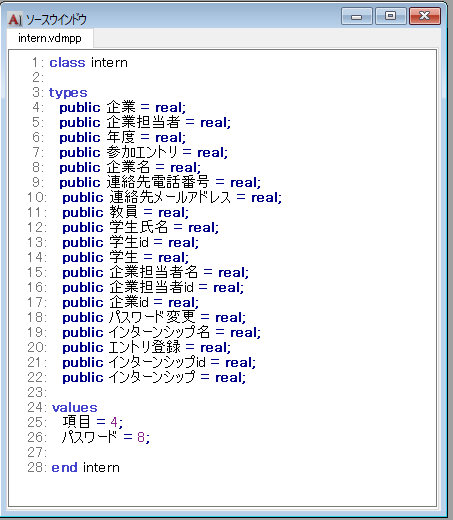
\includegraphics[width=300]{image/exis_vdm.png}
        \caption{既存手法のVDM++仕様書生成処理が生成するVDM++仕様書}
        \label{fig:exis_vdm}
    \end{center}
\end{figure}

\section{既存手法の問題点}
\label{sec:problemm}
既存手法は、上記の4つの処理部によって、自然言語仕様書内の単語の内、VDM++仕様書に必要な単語を抽出し、VDM++仕様書を自動生成することができる。
しかし、既存手法は、自然言語仕様書から抽出した単語を、VDM++仕様書に必要である単語と必要でない単語に分類し、型定義と定数定義に対応したVDM++仕様書を出力できるが、
クラスやその他のブロック定義に対応したVDM++仕様書を出力することができない。そのため、既存手法は、対応しているVDM++の構文が少なく、有用性が低い。
本論文では、既存手法の有用性の向上を目的として、VDM++仕様書における以下の3つの構文を生成する手法を提案する。
さらに、提案手法を既存手法に適用し、機械学習を活用したVDM++仕様書自動生成ツールVGMLを開発する。

\begin{itemize}
    \item クラス
    \item インスタンス変数
    \item 操作定義
\end{itemize}
\chapter{MATCHの実装}\label{cha:Implementation}

Coming soon...

\chapter{適用例}
\label{cha:Indication}

本研究では、既存ツールの問題を解決するために、自然言語仕様書から、
クラス、インスタンス変数定義、操作定義を記述したVDM++仕様書を生成する手法を提案し、
既存ツールに適用することでVGMLを開発した。

適用例では、VGMLに自然言語仕様書を適用することで、クラス、型定義、定数定義、インスタンス変数定義、操作定義を記述したVDM++仕様書を生成できること、
かつ、生成したVDM++仕様書の構文が正しいことを確認する。また、VGMLが教師データの自然言語仕様書と異なる自然言語仕様書に対応できることを確認する。

\section{教師データの自然言語仕様書と同じ自然言語仕様書の適用}
\label{sec:generate_vdm}

VGMLに、Microsoft社のwordで記述した自然言語仕様書「インターンシップ評定書・オンライン提出システム」(付録A.参照)を適用し、VDM++仕様書を生成する。
以降、自然言語仕様書「インターンシップ評定書・オンライン提出システム」を、仕様書Aと表現する。

この適用例では、学習済みモデルを生成するために使用した教師データの自然言語仕様書と同じ自然言語仕様書をVGMLに適用することによって、
VGMLが、VDM++仕様書のクラス、型定義、定数定義、インスタンス変数定義、操作定義を生成できること、かつ、生成したVDM++仕様書の構文が正しいことを確認する。

VGMLに仕様書Aを適用した結果、6つのファイルを生成した。
VGMLが仕様書Aを基に生成した6つのファイルを、図\ref{fig:indication_vdm1}-図\ref{fig:indication_vdm6}に示す。
図\ref{fig:indication_vdm1}-図\ref{fig:indication_vdm6}は、VDM++ Toolbox\cite{Tools}での出力の画面である。

\begin{figure}[p]
    \begin{center}
    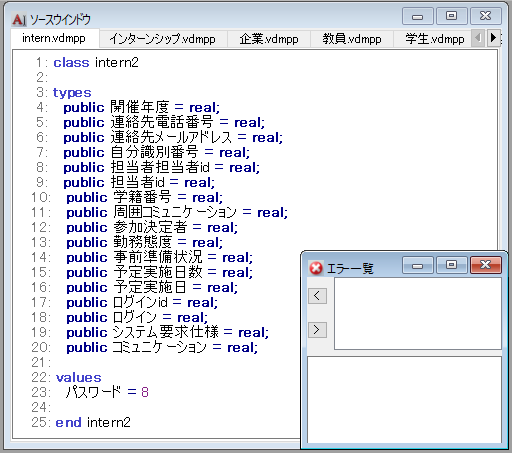
\includegraphics[width=300]{image/indication_vdm1.PNG}
    \caption{VGMLが仕様書Aを基に生成したファイル1}
    \label{fig:indication_vdm1}
    \end{center}
\end{figure}

\begin{figure}[p]
    \begin{center}
    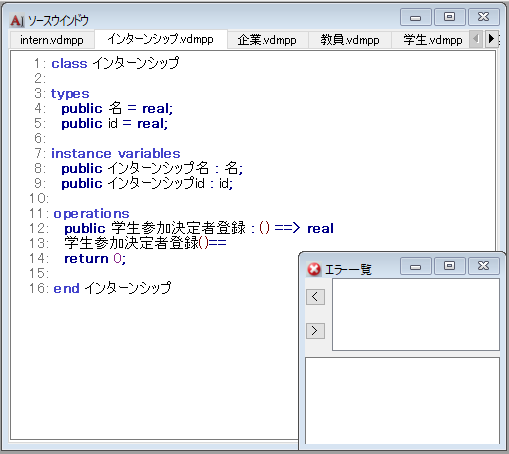
\includegraphics[width=300]{image/indication_vdm2.PNG}
    \caption{VGMLが仕様書Aを基に生成したファイル2}
    \label{fig:indication_vdm2}
    \end{center}
\end{figure}

\begin{figure}[p]
    \begin{center}
    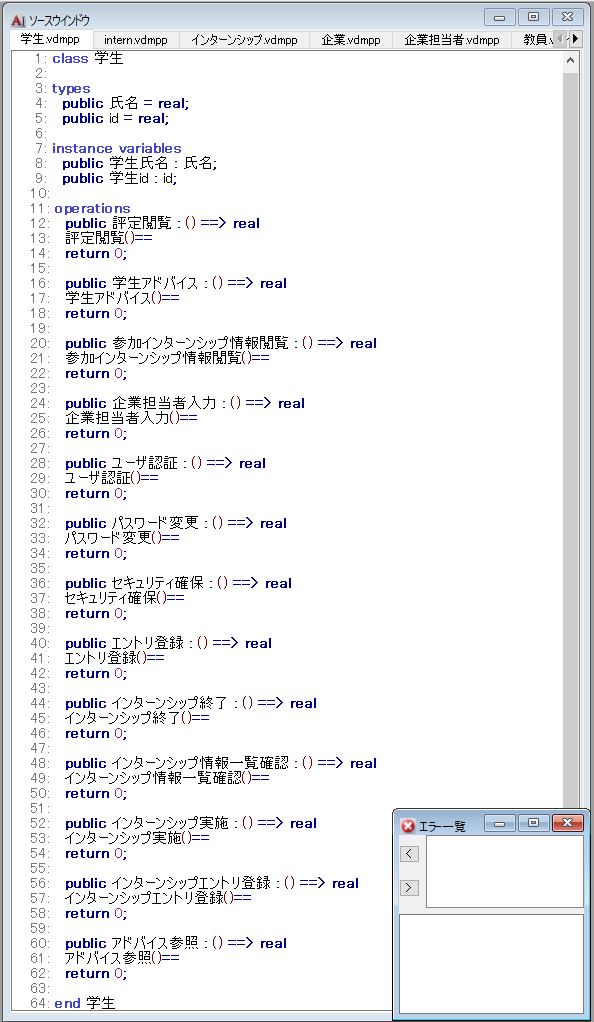
\includegraphics[width=300]{image/indication_vdm3.PNG}
    \caption{VGMLが仕様書Aを基に生成したファイル3}
    \label{fig:indication_vdm3}
    \end{center}
\end{figure}

\begin{figure}[tp]
    \begin{center}
    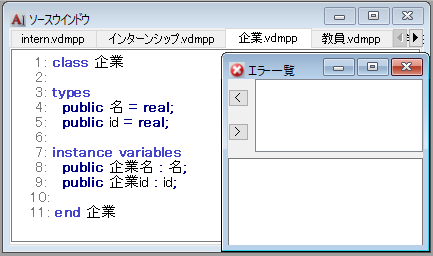
\includegraphics[width=300]{image/indication_vdm4.PNG}
    \caption{VGMLが仕様書Aを基に生成したファイル4}
    \label{fig:indication_vdm4}
    \end{center}
\end{figure}

\begin{figure}[tp]
    \begin{center}
    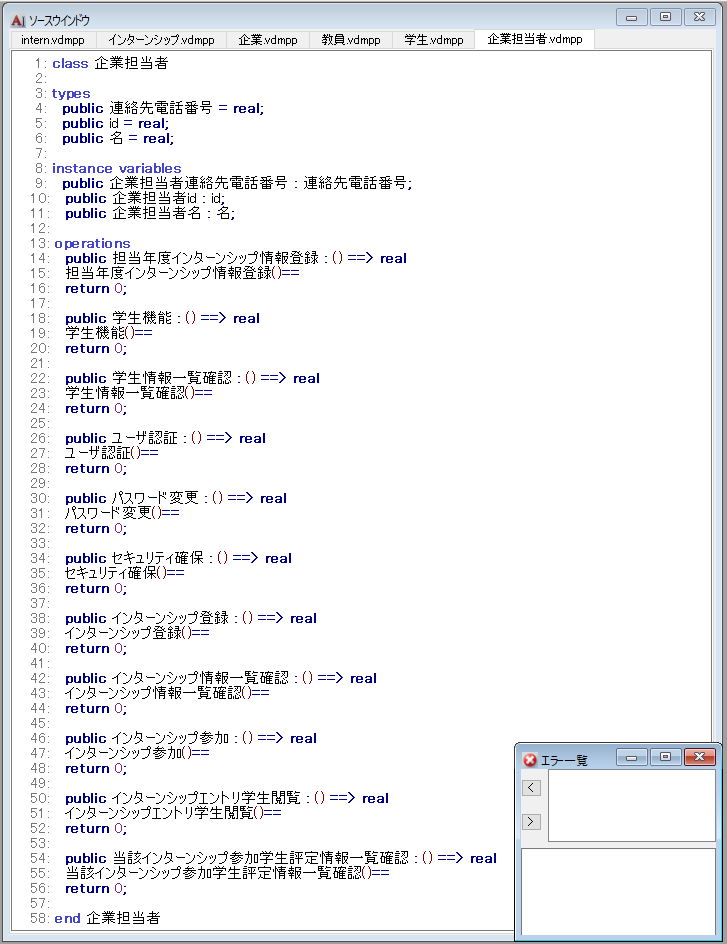
\includegraphics[width=300]{image/indication_vdm5.PNG}
    \caption{VGMLが仕様書Aを基に生成したファイル5}
    \label{fig:indication_vdm1}
    \end{center}
\end{figure}

\begin{figure}[tp]
    \begin{center}
    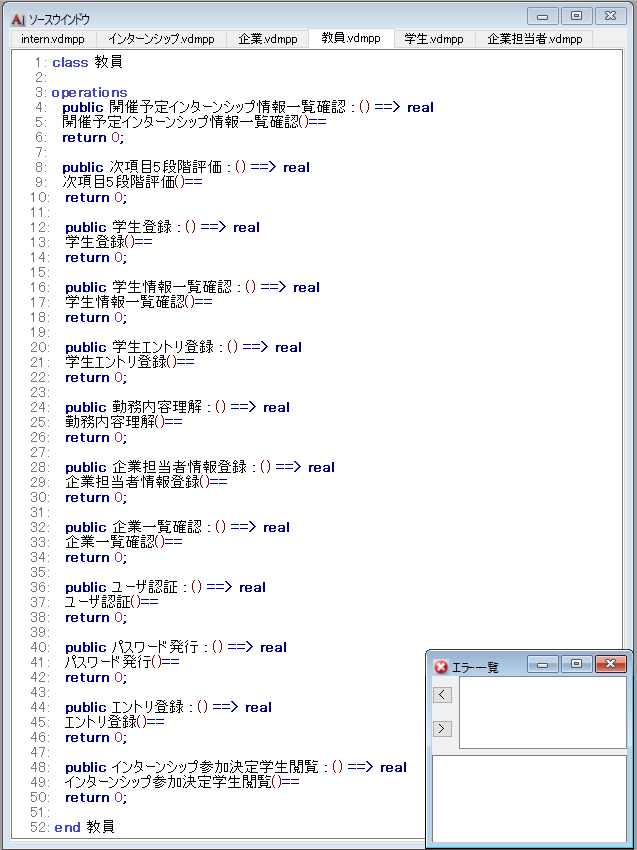
\includegraphics[width=300]{image/indication_vdm6.PNG}
    \caption{VGMLが仕様書Aを基に生成したファイル6}
    \label{fig:indication_vdm6}
    \end{center}
\end{figure}

構文、および、タイプチェッカーを備えたVDM++ Toolboxは、生成したVDM++仕様書に対して警告を表示しなかった。
このことから、VGMLに自然言語仕様書を適用することにより、
クラス、型定義、定数定義、インスタンス変数定義、操作定義を記述したVDM++仕様書を生成できること、
かつ、生成したVDM++仕様書の構文が正しいことを確認した。

\section{教師データの自然言語仕様書と異なる自然言語仕様書の適用}
\label{sec:different_generate_vdm}

VGMLに、pdfで記述した「ETロボコン2020競技規約」\cite{ET_robo}を適用し、VDM++仕様書を生成する。
また、学習済みモデルについては、\ref{sec:vgml_train_model}節で仕様書Aを基に生成した学習済みモデルを使用する。
付録B.に、「ETロボコン2020競技規約」の自然言語仕様書の$4~13$ページ、および、$24~31$ページを示す。
なお、今回対象としなかった$1~3$ページは、目次および仕様書を読むための項目であったため対象から外した。
さらに、「ETロボコン2020」の競技は、3つのクラスに別れており、今回はアドバンストクラスについての自然言語仕様書である$24~31$ページを対象とした。
以降、「ETロボコン2020競技規約」の$24~31$ページを、仕様書Bと表現する。

この適用例では、学習済みモデルを生成するために使用した教師データの自然言語仕様書と異なる自然言語仕様書をVGMLに適用することによって、
VGMLが、教師データの自然言語仕様書と異なる自然言語仕様書に対しても、
VDM++仕様書のクラス、型定義、定数定義、インスタンス変数定義、操作定義を生成できること、かつ、生成したVDM++仕様書の構文が正しいことを確認する。

VGMLに仕様書Bを適用した結果、6つのファイルを生成した。
VGMLが仕様書Bを基に生成した6つのファイルを、図\ref{fig:indicationB_vdm1}-図\ref{fig:indicationB_vdm6}に示す。
図\ref{fig:indicationB_vdm1}-図\ref{fig:indicationB_vdm6}は、VDM++ Toolbox\cite{Tools}での出力の画面である。
構文、および、タイプチェッカーを備えたVDM++ Toolboxは、生成したVDM++仕様書に対して警告を表示しなかった。

\begin{figure}[p]
    \begin{center}
    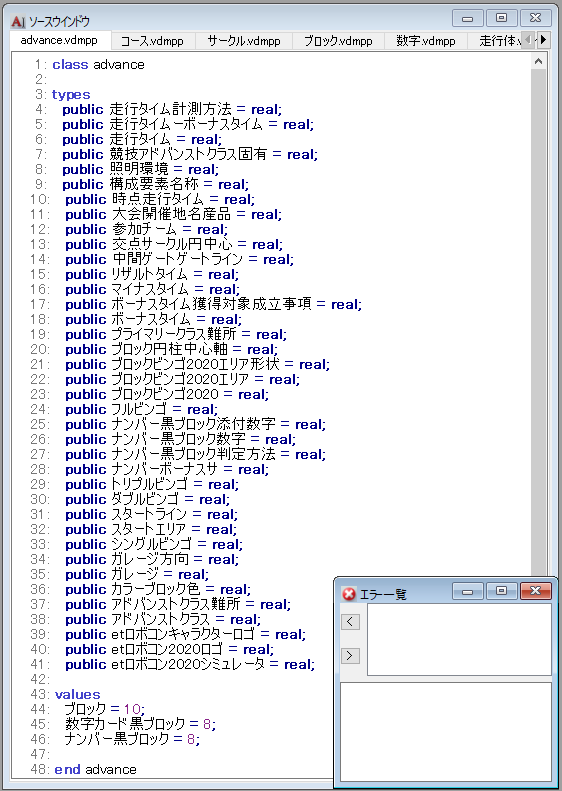
\includegraphics[width=300]{image/indicationB_vdm1.PNG}
    \caption{VGMLが仕様書Bを基に生成したファイル1}
    \label{fig:indicationB_vdm1}
    \end{center}
\end{figure}

\begin{figure}[p]
    \begin{center}
    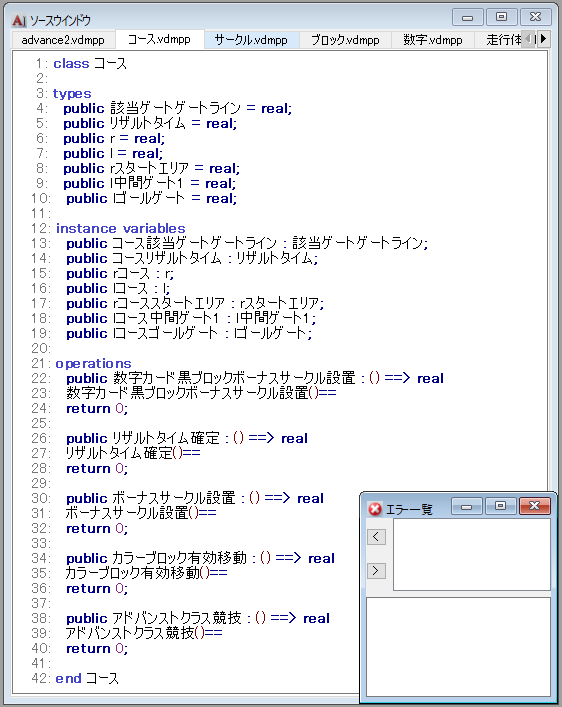
\includegraphics[width=300]{image/indicationB_vdm2.PNG}
    \caption{VGMLが仕様書Bを基に生成したファイル2}
    \label{fig:indicationB_vdm2}
    \end{center}
\end{figure}

\begin{figure}[p]
    \begin{center}
    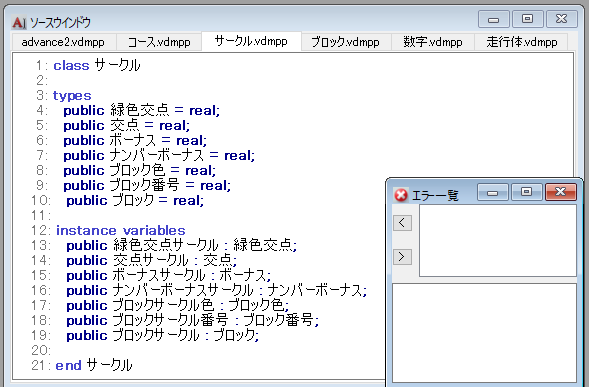
\includegraphics[width=300]{image/indicationB_vdm3.PNG}
    \caption{VGMLが仕様書Bを基に生成したファイル3}
    \label{fig:indicationB_vdm3}
    \end{center}
\end{figure}

\begin{figure}[tp]
    \begin{center}
    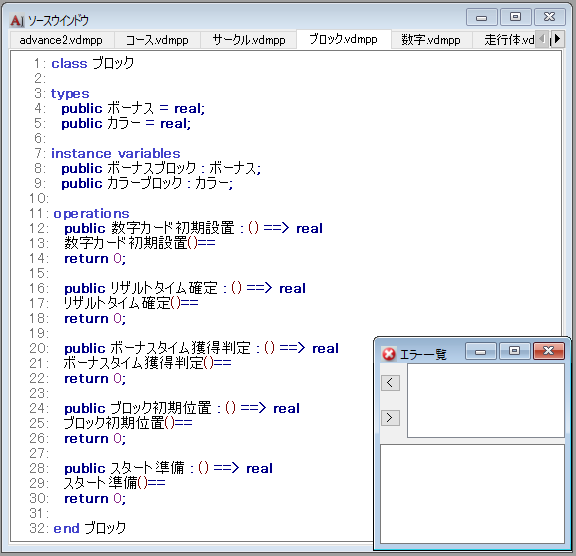
\includegraphics[width=300]{image/indicationB_vdm4.PNG}
    \caption{VGMLが仕様書Bを基に生成したファイル4}
    \label{fig:indicationB_vdm4}
    \end{center}
\end{figure}

\begin{figure}[tp]
    \begin{center}
    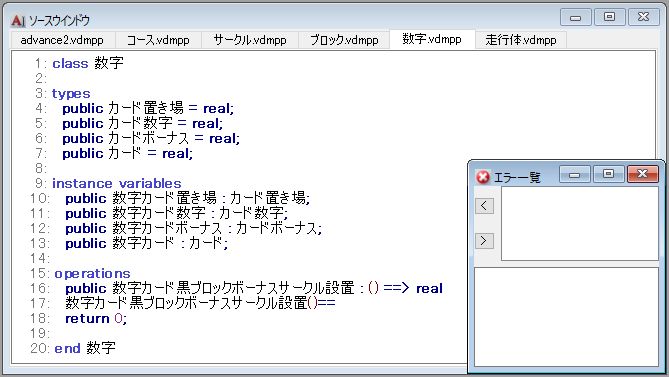
\includegraphics[width=300]{image/indicationB_vdm5.PNG}
    \caption{VGMLが仕様書Bを基に生成したファイル5}
    \label{fig:indicationB_vdm5}
    \end{center}
\end{figure}

\begin{figure}[tp]
    \begin{center}
    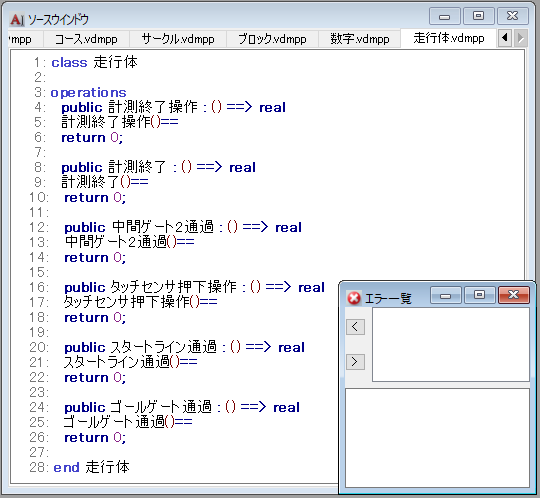
\includegraphics[width=300]{image/indicationB_vdm6.PNG}
    \caption{VGMLが仕様書Bを基に生成したファイル6}
    \label{fig:indicationB_vdm6}
    \end{center}
\end{figure}

このことから、VGMLに学習済みモデルを生成するために使用した教師データの自然言語仕様書と異なる自然言語仕様書を適用することにより、
学習済みモデルが教師データの自然言語仕様書と異なる自然言語仕様書に対しても、
VDM++仕様書のクラス、型定義、定数定義、インスタンス変数定義を生成できること、
かつ、生成したVDM++仕様書の構文が正しいことを確認した。

以上、\ref{sec:generate_vdm}節と\ref{sec:different_generate_vdm}節の適用結果により、VGMLが
VDM++仕様書のクラス、型定義、定数定義、インスタンス変数定義、操作定義を生成できること、かつ、生成したVDM++仕様書の構文が正しいことを確認した。
\chapter{考察}
\label{cha:Discussion}

本研究では、既存ツールの有用性の向上を目的として、自然言語仕様書からクラス、操作定義、操作定義を生成する手法を提案し、
既存ツールに適用することによってVGMLを開発した。
本章では、VGMLに関して考察する。

\section{VGMLの有用性}
本節では、VGMLが自然言語仕様書から生成したVDM++仕様書を、正解のVDM++仕様書と比較して評価する。ここで、正解のVDM++仕様書として、
著者が仕様書Aと仕様書Bから人手によって記述したVDM++仕様書を用いる。
仕様書Aから人手によって記述したVDM++仕様書は、6つのファイルで構成し、仕様書Bから人手によって記述したVDM++仕様書は、7つのファイルで構成する。
仕様書Aから作成したVDM++仕様書を、図\ref{fig:speA_vdm1}-図\ref{fig:speA_vdm6}に、仕様書Bから作成したVDM++仕様書を、図\ref{fig:speB_vdm1}-図\ref{fig:speB_vdm7}に示す。

正解のVDM++仕様書は、以下の条件に基づいて作成した。

\begin{itemize}
    \item 自然言語仕様書内で属性や振る舞いを持ち、自然言語仕様書が対象とするシステムの外部に位置するアクターではない名詞を、クラスとして定義する。
    \item システム内で数字などの不変の情報を持つ名詞を定数名とし、当該名詞が持つ情報を値として定義する。
    \item あるクラスの候補となる名詞が持つ情報であり、クラスが振る舞いを行う際に必要とする情報である名詞を、当該クラスの候補である名詞の持つインスタンス変数として定義する。
    \item あるクラスの候補となる名詞が行う振る舞いを表す名詞であり、かつ、操作定義の候補である名詞を参照する名詞。
\end{itemize}

今回は、VGMLの有用性の評価のために、VGMLが生成したVDM++仕様書内の単語と、正解のVDM++仕様書内の単語についてのF値を測定した。
F値は、適合率と再現率の調和平均である。F値の計算式を、以下に示す。

\begin{equation}
    \mbox F値=\frac{2 \times 適合率 \times 再現率}{適合率+再現率}
\end{equation}	

評価する項目を、以下に示す。

\begin{itemize}
    \item クラスに対する評価
    \item インスタンス変数定義に対する評価
    \item 操作定義に対する評価
\end{itemize}

以降、それぞれの評価について示す。

\subsection{クラスに対する評価}
VGMLが生成するVDM++仕様書におけるクラスと、正解のVDM++仕様書におけるクラスを比較し、一致したクラスをF値を用いて評価する。
クラスに対する評価の適合率は、VGMLが生成したクラスのうち、正解のVDM++仕様書のクラスと一致したクラスの数との割合であり、
再現率は正解のVDM++仕様書のクラスのうち、VGMLが生成したクラスと一致したクラスの数との割合である。
以下に、クラスに対する評価の適合率、再現率の計算式を、それぞれ示す。

\begin{equation}
    \mbox 適合率=\frac{正解の\mathrm{VDM\!+\!+}仕様書のクラスと一致したクラスの数}{VGMLが出力したクラスの数}
\end{equation}
\begin{equation}
    \mbox 再現率=\frac{正解の\mathrm{VDM\!+\!+}仕様書のクラスと一致したクラスの数}{正解の\mathrm{VDM\!+\!+}仕様書のクラスの数}
\end{equation}

VGMLが生成したVDM++仕様書におけるクラスと、正解のVDM++仕様書におけるクラスを比較した際の実験結果を、表\ref{table:classResult}に示す。

表\ref{table:classResult}より、VGMLは、抽出した単語をクラスとして出力する際に、仕様書AでF値1.0、仕様書BでF値0.72の精度で出力できた。
このことにより、VGMLは、教師データの自然言語仕様書と異なる自然言語仕様書に対しても、一定の割合でVDM++仕様書におけるクラスを生成できることがわかる。
よって、VGMLは、既存ツールの有用性を向上できたといえる。


\begin{table}[t]
	\caption{VGMLが生成したVDM++仕様書におけるクラスと正解のVDM++仕様書におけるクラスを比較した際の実験結果}
	\label{table:classResult}
	\begin{center}
        \begin{tabular}{c|c|c|c|c|c|c}
            \hline
            仕様書  & 正解の & 出力した & 一致した & 適合率 & 再現率 & F値  \\
                    & VDM++仕様書 & VDM++仕様書 &         &        &       &      \\
                    & のクラスの数 & のクラスの数 & クラスの数  &        &       &      \\
            \hline
            仕様書A & 5                             & 5                 & 5                  & 1.0   & 1.0    & 1.0  \\
            \hline
            仕様書B & 6                             & 5                  & 4                  & 0.8   & 0.67   & 0.72 \\
            \hline
        \end{tabular}
    \end{center}
\end{table}

\subsection{インスタンス変数定義に対する評価}
VGMLが生成するVDM++仕様書におけるインスタンス変数定義と、正解のVDM++仕様書におけるインスタンス変数定義を比較し、一致したインスタンス変数定義をF値を用いて評価する。
インスタンス変数定義に対する評価の適合率は、VGMLが生成したインスタンス変数定義のうち、正解のVDM++仕様書のインスタンス変数定義と一致したインスタンス変数定義の数との割合であり、
再現率は正解のVDM++仕様書のインスタンス変数定義のうち、VGMLが生成したインスタンス変数定義と一致したインスタンス変数定義の数との割合である。
以下に、インスタンス変数定義に対する評価の適合率、再現率の計算式を、それぞれ示す。

\begin{equation}
    \mbox 適合率=\frac{正解の\mathrm{VDM\!+\!+}仕様書のインスタンス変数定義と一致したインスタンス変数定義の数}{VGMLが出力したインスタンス変数定義の数}
\end{equation}
\begin{equation}
    \mbox 再現率=\frac{正解の\mathrm{VDM\!+\!+}仕様書のインスタンス変数定義と一致したインスタンス変数定義の数}{正解の\mathrm{VDM\!+\!+}仕様書のインスタンス変数定義の数}
\end{equation}

VGMLが生成したVDM++仕様書におけるインスタンス変数定義と、正解のVDM++仕様書におけるインスタンス変数定義を比較した際の実験結果を、表\ref{table:classResult}に示す。

表\ref{table:instanceResult}より、VGMLは、抽出した単語をインスタンス変数定義として出力する際に、仕様書AでF値0.62、仕様書BでF値0.61の精度で出力できた。
このことにより、VGMLは、教師データの自然言語仕様書と異なる自然言語仕様書に対しても、一定の割合でVDM++仕様書におけるインスタンス変数定義を生成できることがわかる。
よって、VGMLは、既存ツールの有用性を向上できたといえる。

\begin{table}[t]
	\caption{VGMLが生成したVDM++仕様書におけるインスタンス変数定義と正解のVDM++仕様書におけるインスタンス変数定義を比較した際の実験結果}
	\label{table:instanceResult}
	\begin{center}
        \begin{tabular}{c|c|c|c|c|c|c}
            \hline
            仕様書  & 正解の & 出力した &  & 適合率 & 再現率 & F値  \\
                    & VDM++仕様書の & VDM++仕様書の & 一致した  &        &       &      \\
                    & インスタンス & インスタンス & インスタンス  &        &       &      \\
                    & 変数定義の数 & 変数定義の数 & 変数定義の数  &        &       &      \\
            \hline
            仕様書A & 20                             & 10                 & 9                  & 0.9   & 0.45    & 0.62  \\
            \hline
            仕様書B & 26                             & 20                  & 14                  & 0.7   & 0.54   & 0.61 \\
            \hline
        \end{tabular}
    \end{center}
\end{table}

\subsection{操作定義に対する評価}
VGMLが生成するVDM++仕様書における操作定義と、正解のVDM++仕様書における操作定義を比較し、一致した操作定義をF値を用いて評価する。
操作定義に対する評価の適合率は、VGMLが生成した操作定義のうち、正解のVDM++仕様書の操作定義と一致した操作定義の数との割合であり、
再現率は正解のVDM++仕様書の操作定義のうち、VGMLが生成した操作定義と一致した操作定義の数との割合である。
以下に、操作定義に対する評価の適合率、再現率の計算式を、それぞれ示す。

\begin{equation}
    \mbox 適合率=\frac{正解の\mathrm{VDM\!+\!+}仕様書の操作定義と一致した操作定義の数}{VGMLが出力した操作定義の数}
\end{equation}
\begin{equation}
    \mbox 再現率=\frac{正解の\mathrm{VDM\!+\!+}仕様書の操作定義と一致した操作定義の数}{正解の\mathrm{VDM\!+\!+}仕様書の操作定義の数}
\end{equation}

VGMLが生成したVDM++仕様書における操作定義と、正解のVDM++仕様書における操作定義を比較した際の実験結果を、表\ref{table:classResult}に示す。

表\ref{table:operateResult}より、VGMLは、抽出した単語を操作定義として出力する際に、仕様書AでF値0.68、仕様書BでF値0.54の精度で出力できた。
このことにより、VGMLは、教師データの自然言語仕様書と異なる自然言語仕様書に対しても、一定の割合でVDM++仕様書における操作定義を生成できることがわかる。
よって、VGMLは、既存ツールの有用性を向上できたといえる。

\begin{table}[t]
	\caption{VGMLが生成したVDM++仕様書における操作定義と正解のVDM++仕様書における操作定義を比較した際の実験結果}
	\label{table:operateResult}
	\begin{center}
        \begin{tabular}{c|c|c|c|c|c|c}
            \hline
            仕様書  & 正解の & 出力した &  & 適合率 & 再現率 & F値  \\
                    & VDM++仕様書の & VDM++仕様書の & 一致した  &        &       &      \\
                    & 操作定義の数 & 操作定義の数 & 操作定義の数  &        &       &      \\
            \hline
            仕様書A & 31                             & 37                 & 23                  & 0.63   & 0.74    & 0.68  \\
            \hline
            仕様書B & 16                             & 17                  & 9                  & 0.53   & 0.56   & 0.54 \\
            \hline
        \end{tabular}
    \end{center}
\end{table}

\section{関連研究}
自然言語仕様書からVDM++仕様書を生成する研究として、大森氏らの研究\cite{research1,research2}がある。
この研究では、自然言語仕様書と形式モデルの相互変換をサポートし、対応付けを辞書として管理する辞書ツールを開発することによって、
自然言語仕様書からVDM++仕様書を生成できる\cite{research1}。
辞書ツールに自然言語仕様書内の単語を辞書として登録し、登録した単語を類義語やグループ分けの定義や状態として定義することにより、
自然言語仕様書に含まれる曖昧さをなくすことができる。また、入力となる形式的定義と出力する形式的種別を辞書ツールに登録しておくことで、
VDM++仕様書を生成できる。さらに、辞書ツールを使用した形式仕様の作成から実装までを行うことで形式仕様への変換の手順の改良を提案した\cite{research2}。
これによって、辞書ツールを使用した自然言語仕様書から形式仕様の手順を適用することで発生する問題点と、この手順を適用する際に考慮すべき点が発見できた。
大森氏らが開発した辞書ツールが、自然言語仕様書からVDM++仕様書の作成を支援するツールであること対し、VGMLは、機械学習を用いて自然言語仕様書から
VDM++仕様書を自動で生成できる。さらに、VGMLは、既存ツールの型定義と定数定義に加え、クラス、インスタンス変数定義、操作定義の生成が可能である。
また、英語の自然言語仕様書を入力とし、VDM++仕様書を自動生成する研究として、Lee氏らの研究がある\cite{research3}。
この研究は、英語の要件ドキュメントから形式仕様記述への変換の自動化を目的として、形式仕様記述と言語技術のアプリケーションを提案した。
このアプリケーションは、適切に構造化されたテキストを使用して、英語の要件から知識ベースに変換する。
知識ベースは、英語の要件ドキュメントから構成する。
また、知識ベースからTLG(Two Level Grammar)に変換する。
さらに、自然言語処理によって英語の自然言語仕様書とTLGのあいまいさを処理し、英語の要件ドキュメントから異なる形式を持つ形式仕様言語を生成できる。
この研究は、単語ごとに意味を解析することによって、英語の自然言語仕様書からVDM++仕様書を自動生成できる。
しかし、日本語の自然言語仕様書の場合は、文章が単語ごとに分ち書きされていない、かつ、1つの単語だけでは意味を持たない可能性があるため、
日本語の自然言語仕様書にそのまま適用することはできない。
これに対し、VGMLは、日本語の自然言語仕様書を対象として、形態素解析によって自然言語仕様書内の文を分かち書きし、
機械学習によって、分かち書きした単語をUNNECESSARY、NONCLASS、CLASSのいずれかに分類する。
さらに、分類した単語をVDM++の構文に当てはめて出力することによって、VDM++仕様書を自動で生成する。
これは、日本語の仕様書を入力として、VDM++仕様書を自動で生成したという点に関して、本研究が初である。

\section{VGMLの問題点}
本研究で開発したVGMLの問題点を、以下に示す。

\begin{itemize}
	\item 関数定義に対応していない\\VGMLは、VDM++を構成するブロックである関数定義には対応していない。この問題については、形態素解析を用いて本研究で抽出した振る舞いを表す単語を、インスタンス変数の候補である単語と関係するか否かの条件を基に分類することで対応できると考える。
	\item 制約条件の記述への対応\\本研究は、自然言語仕様書からVDM++仕様書を生成することを目的としてるが、VGMLが生成するVDM++仕様書は、VDM++仕様書において重要である事前条件、事後条件、不変条件といった制約条件の記述に対応できていない。この問題については、自然言語仕様書内の「最大」、「未満」、「以内」といった範囲を表す単語を抽出し、制約条件として記述するアルゴリズムを提案する必要がある。
	\item 型定義と定数定義の要素のクラスの候補となる単語への分類\\VGMLは、既存ツールで抽出した型・定数定義の候補である単語を、クラスの候補となる単語へ分類することができない。この問題については、抽出したクラスの候補である単語を多項ロジスティック回帰分析における目的変数とし、型・定数定義の候補である単語を、機械学習を用いてクラスに分類することで対応できると考える。
	\item VDM++仕様書のreal型以外の型への対応\\VGMLは、VDM++における型定義を生成する際に、実数型であるreal型しか出力できないため、より厳密な仕様書を生成することができない。この問題については、VGMLが生成する数値リスト内の数値の条件を表す表現を自然言語仕様書内から解析することによって対応できると考える。
\end{itemize}

\begin{figure}[tp]
    \begin{center}
    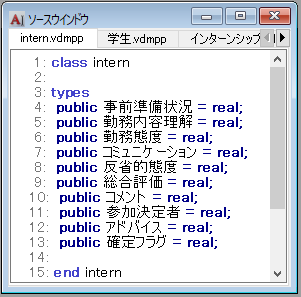
\includegraphics[width=300]{image/speA_vdm1.PNG}
    \caption{仕様書Aから人手によって生成したファイル1}
    \label{fig:speA_vdm1}
    \end{center}
\end{figure}

\begin{figure}[tp]
    \begin{center}
    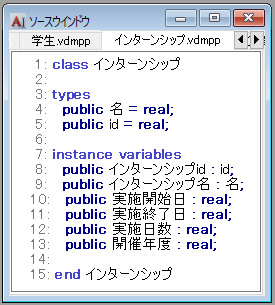
\includegraphics[width=300]{image/speA_vdm2.PNG}
    \caption{仕様書Aから人手によって生成したファイル2}
    \label{fig:speA_vdm2}
    \end{center}
\end{figure}

\begin{figure}[tp]
    \begin{center}
    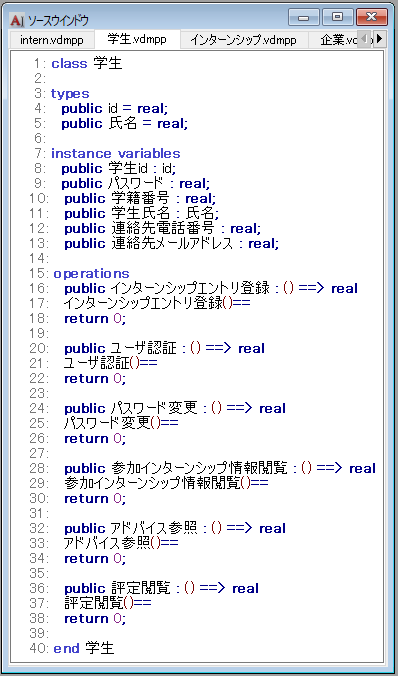
\includegraphics[width=300]{image/speA_vdm3.PNG}
    \caption{仕様書Aから人手によって生成したファイル3}
    \label{fig:speA_vdm3}
    \end{center}
\end{figure}

\begin{figure}[tp]
    \begin{center}
    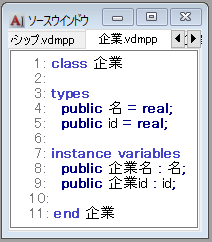
\includegraphics[width=300]{image/speA_vdm4.PNG}
    \caption{仕様書Aから人手によって生成したファイル4}
    \label{fig:speA_vdm4}
    \end{center}
\end{figure}

\begin{figure}[tp]
    \begin{center}
    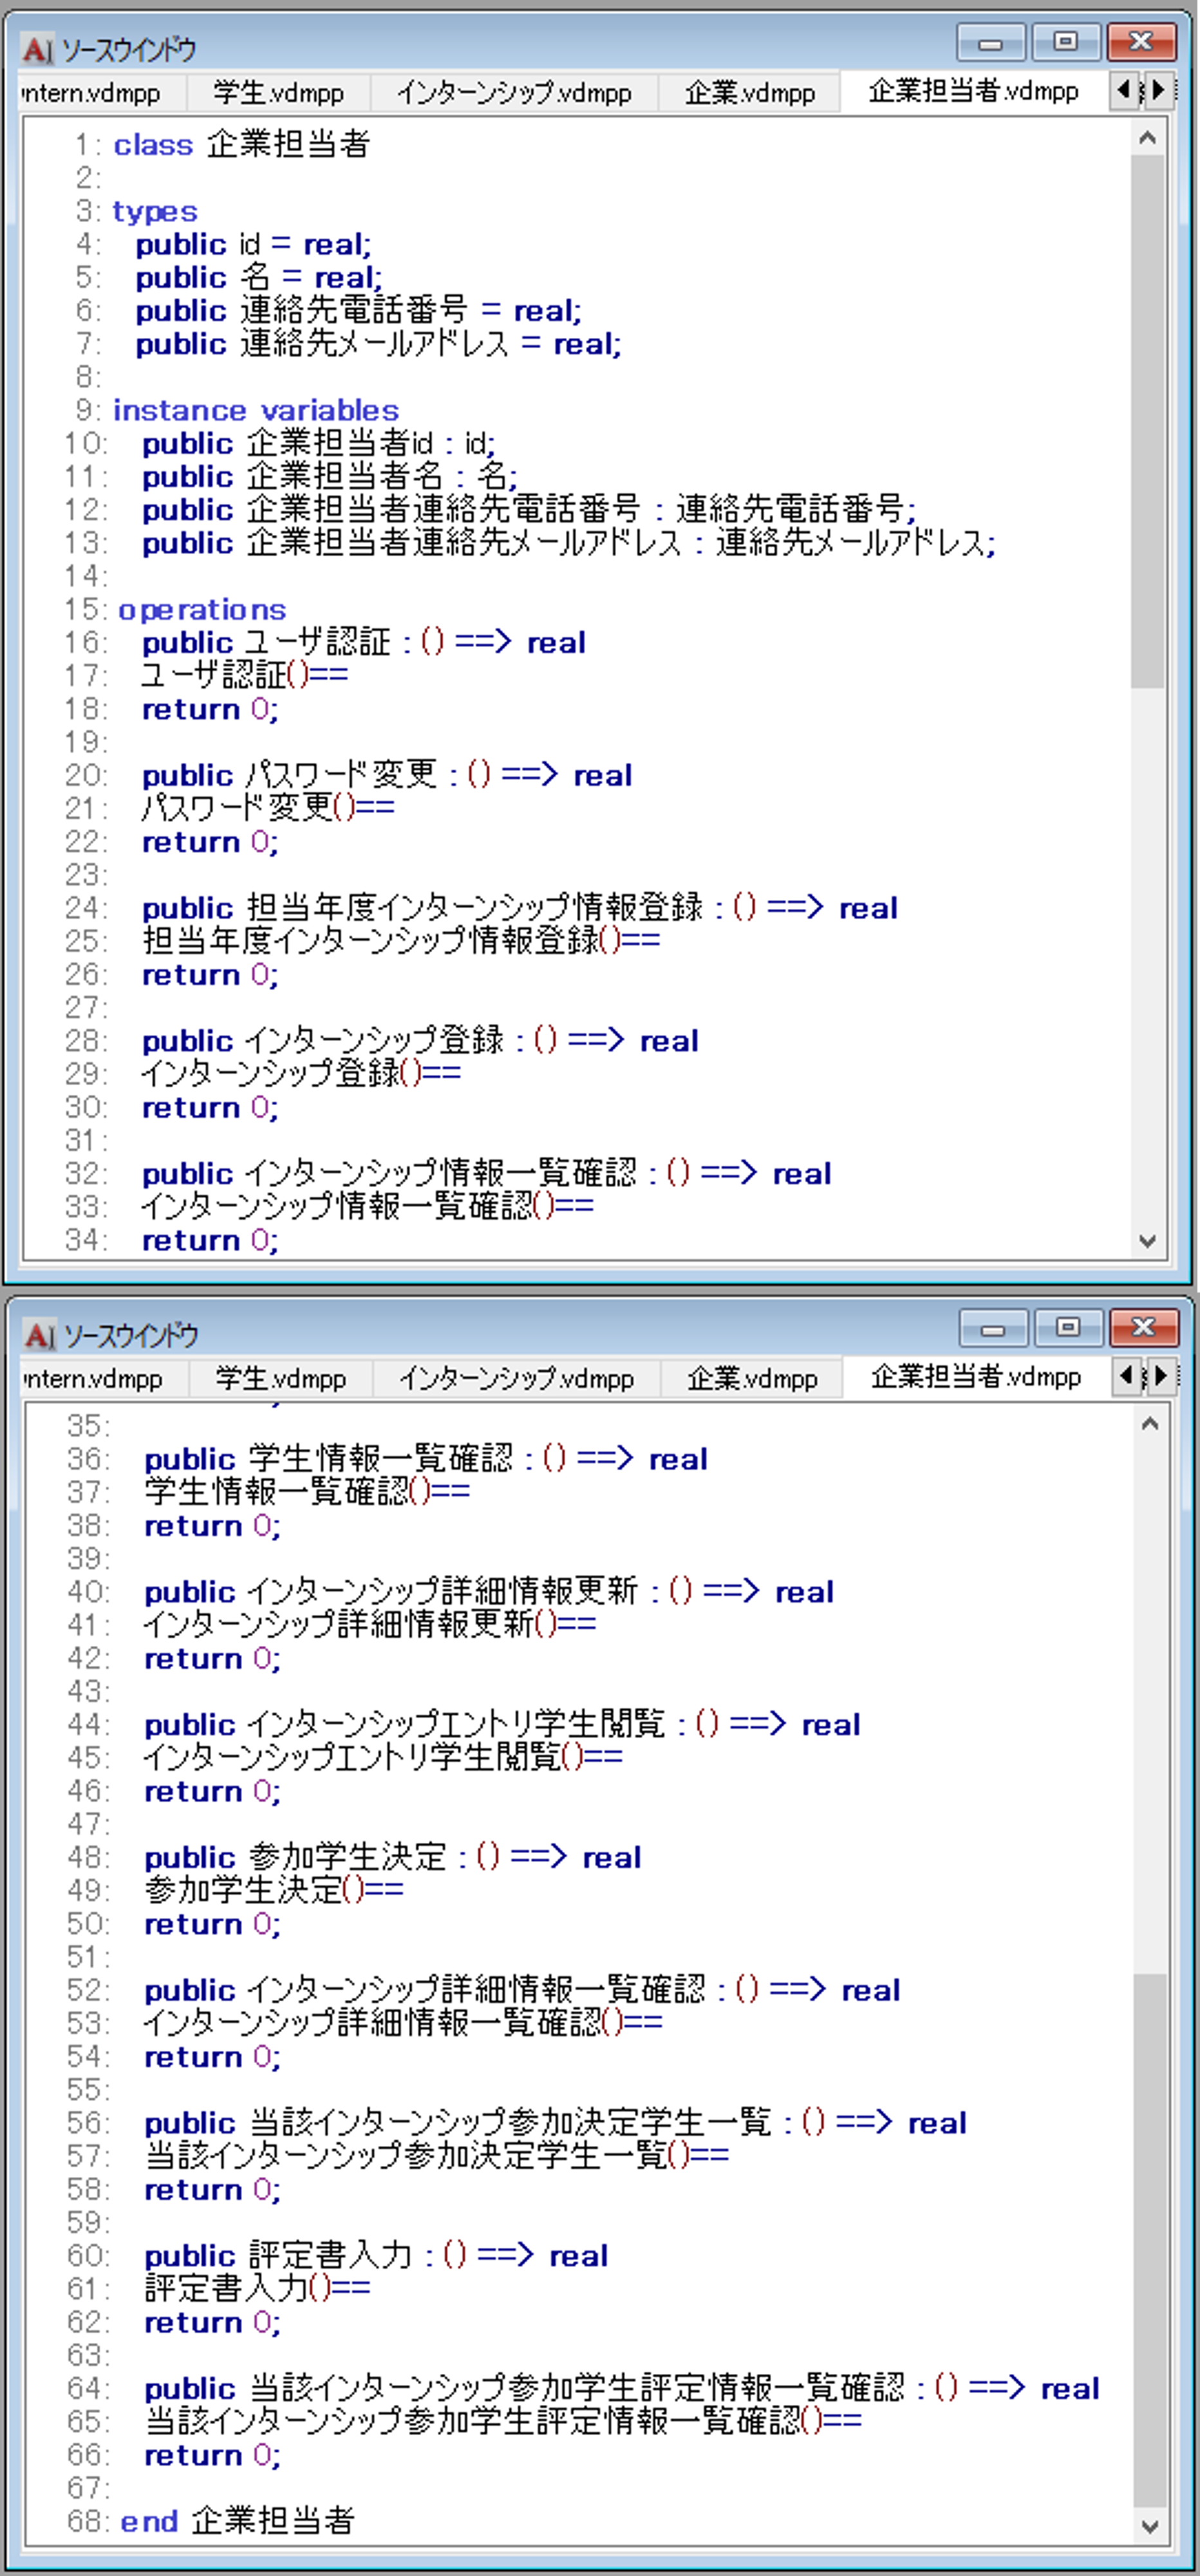
\includegraphics[width=300]{image/speA_vdm5.PNG}
    \caption{仕様書Aから人手によって生成したファイル5}
    \label{fig:speA_vdm5}
    \end{center}
\end{figure}

\begin{figure}[tp]
    \begin{center}
    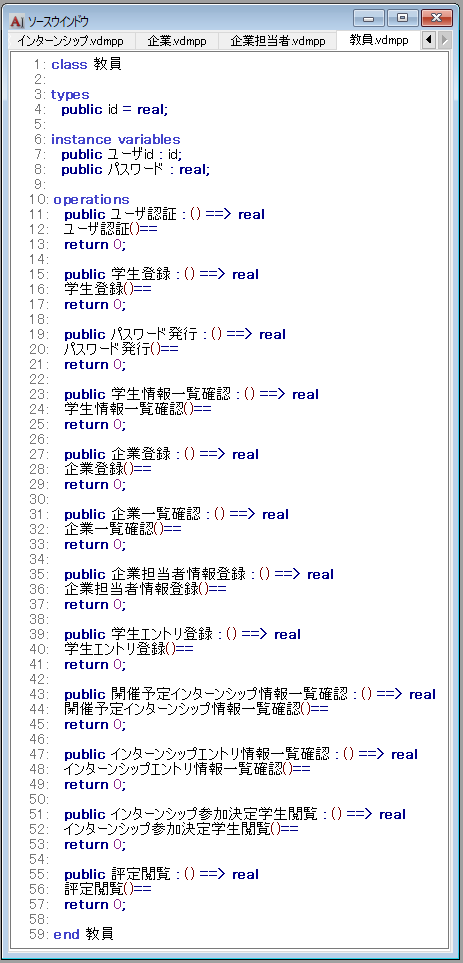
\includegraphics[width=300]{image/speA_vdm6.PNG}
    \caption{仕様書Aから人手によって生成したファイル6}
    \label{fig:speA_vdm6}
    \end{center}
\end{figure}

\begin{figure}[tp]
    \begin{center}
    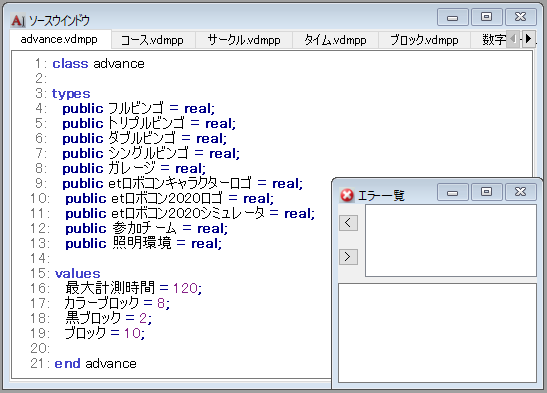
\includegraphics[width=300]{image/speB_vdm1.PNG}
    \caption{仕様書Bから人手によって生成したファイル1}
    \label{fig:speB_vdm1}
    \end{center}
\end{figure}

\begin{figure}[tp]
    \begin{center}
    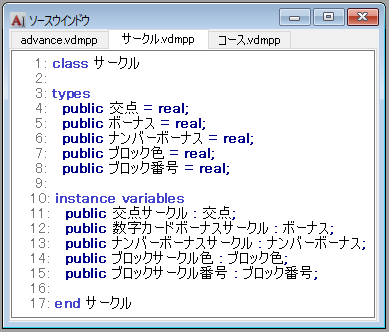
\includegraphics[width=300]{image/speB_vdm2.PNG}
    \caption{仕様書Bから人手によって生成したファイル2}
    \label{fig:speB_vdm2}
    \end{center}
\end{figure}

\begin{figure}[tp]
    \begin{center}
    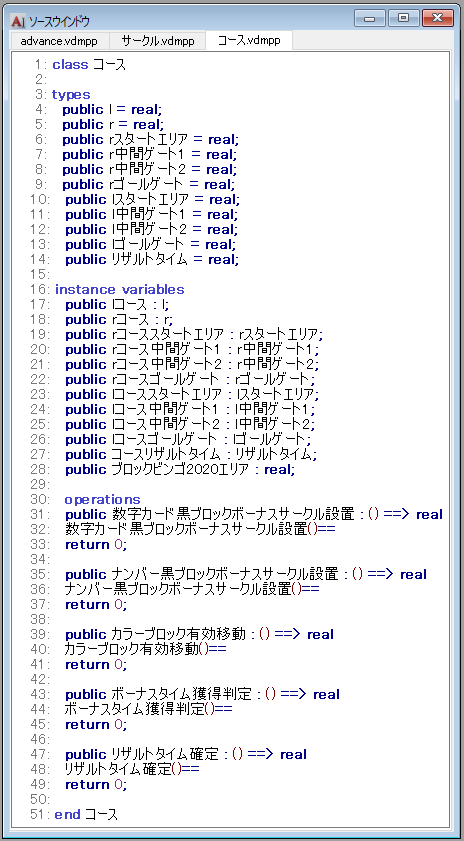
\includegraphics[width=300]{image/speB_vdm3.PNG}
    \caption{仕様書Bから人手によって生成したファイル3}
    \label{fig:speB_vdm3}
    \end{center}
\end{figure}

\begin{figure}[tp]
    \begin{center}
    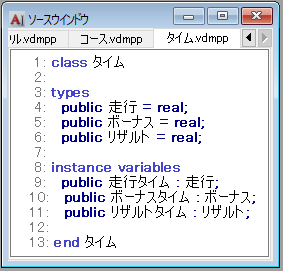
\includegraphics[width=300]{image/speB_vdm4.PNG}
    \caption{仕様書Bから人手によって生成したファイル4}
    \label{fig:speB_vdm4}
    \end{center}
\end{figure}

\begin{figure}[tp]
    \begin{center}
    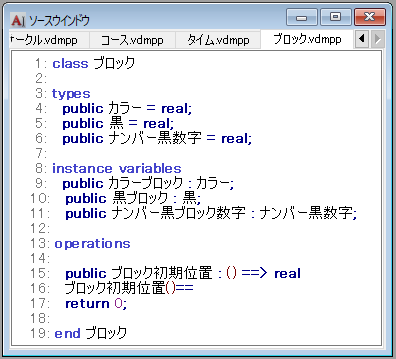
\includegraphics[width=300]{image/speB_vdm5.PNG}
    \caption{仕様書Bから人手によって生成したファイル5}
    \label{fig:speB_vdm5}
    \end{center}
\end{figure}

\begin{figure}[tp]
    \begin{center}
    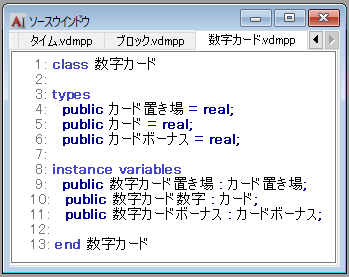
\includegraphics[width=300]{image/speB_vdm6.PNG}
    \caption{仕様書Bから人手によって生成したファイル6}
    \label{fig:speB_vdm6}
    \end{center}
\end{figure}

\begin{figure}[tp]
    \begin{center}
    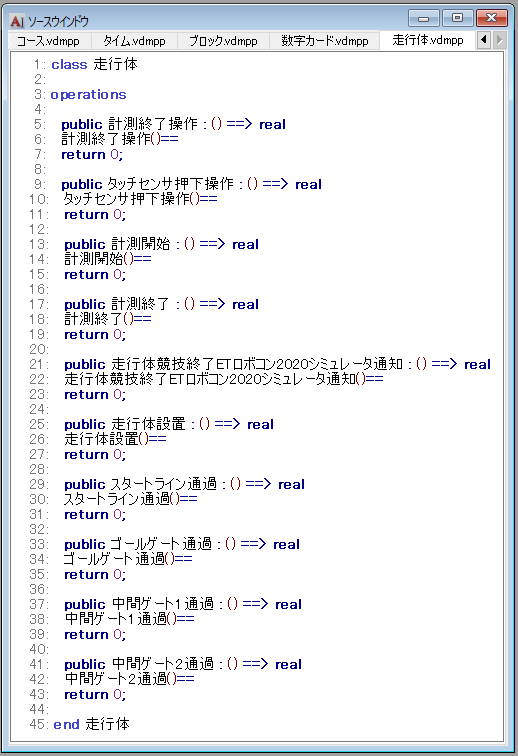
\includegraphics[width=300]{image/speB_vdm7.PNG}
    \caption{仕様書Bから人手によって生成したファイル7}
    \label{fig:speB_vdm7}
    \end{center}
\end{figure}



\chapter{おわりに}\label{cha:Conclusion}

本研究では、既存ツールの有用性の向上を目的として、VDM++仕様書におけるクラス、インスタンス変数定義、操作定義の3つを生成する手法を提案した。
さらに、提案手法を既存ツールに適用し、機械学習を活用したVDM++仕様書自動生成ツールVGMLを開発した。
具体的には、まず、クラスへの対応として、本研究で新たに定義する概念レベルを自然言語仕様書内の単語に対して算出し、機械学習に必要なパラメータとして追加した。
さらに、機械学習を用いて自然言語仕様書内の単語を、UNNECESSARY、NONCLASS、CLASSの3つに分類することでクラスの候補である単語を抽出した。
次に、インスタンス変数定義への対応として、クラスの候補である単語と、クラスの候補である単語に接続する単語の概念レベルを比較することによって、
インスタンス変数定義の候補である単語を抽出した。
次に、操作定義への対応として、VDM++仕様書に必要であるが、クラスの候補ではない単語の内、動詞を表す単語を抽出し、クラスの候補である単語と
抽出した動詞の自然言語仕様書内での関係を解析することによって操作定義の候補である単語を抽出した。
最後に、抽出した各定義ブロックの候補である単語を、VDM++仕様書に記述することで、クラス、型定義、定数定義、インスタンス変数定義、操作定義を記述した
VDM++仕様書を生成した。

適用例として、本研究で開発したVGMLに対して仕様書Aと仕様書Bの2つの自然言語仕様書を適用した。
その結果、VGMLによって、自然言語仕様書から機械学習を用いてVDM++仕様書のクラス、型定義、定数定義、インスタンス変数定義、操作定義を自動生成できること、
かつ、生成したVDM++仕様書の構文が正しいことを確認できた。

また、有用性の評価のために、VGMLが生成したVDM++仕様書と人手によって記述したVDM++仕様書を比較し、
クラス、インスタンス変数定義、操作定義に対してF値を用いて評価した。
評価の結果、まず、VGMLは、自然言語仕様書から抽出した単語をクラスとしてVDM++仕様書に記述する際に、仕様書AでF値1.0、仕様書BでF値0.72
の精度で記述できることを確認した。
次に、VGMLは、自然言語仕様書から抽出した単語をインスタンス変数定義としてVDM++仕様書に記述する際に、仕様書AでF値0.62、仕様書BでF値0.61
の精度で記述できることを確認した。
最後に、VGMLは、自然言語仕様書から抽出した単語を操作定義としてVDM++仕様書に記述する際に、仕様書AでF値0.68、仕様書BでF値0.54
の精度で記述できることを確認した。
このことにより、VGMLは、教師データの自然言語仕様書と同じ自然言語仕様書と、異なる自然言語仕様書に対しても、
一定の割合でクラス、型定義、定数定義、インスタンス変数定義、操作定義を記述したVDM++仕様書を自動生成でき、
既存ツールから、対応するVDM++の構文を増やすことができたといえる。

以上から、VGMLは、既存ツールの有用性を向上できたといえる。

以下に、今後の課題を示す。

\begin{itemize}
	\item 関数定義に対応していない\\VGMLは、VDM++を構成する定義ブロックの1つである関数定義には対応していない。これによって、自然言語仕様書が対象とするシステムにおいて、振る舞いを表す名詞が、インスタンス変数を参照するか否かの判定ができないため、対応する必要がある。
	\item VDM++における制約条件に対応していない\\本研究は、自然言語仕様書からVDM++仕様書を生成することを目的としてる。しかし、VGMLが生成するVDM++仕様書は、VDM++仕様書において重要である事前条件、事後条件、不変条件といった制約条件の記述に対応できていない。これらの制約条件は、VDM++仕様書において重要となる要素であるため、対応する必要がある。
	\item 型・定数定義の候補である単語をクラスの候補となる単語へ分類できていない\\VGMLは、抽出した型・定数定義の候補である単語を、クラスの候補となる単語へ分類できない。これによって、どのクラスが責任を持つ型定義および定数定義かの判定ができないため、対応する必要がある。
	\item VDM++仕様書のreal型以外の型に対応していない\\VGMLは、VDM++における型定義を生成する際に、実数型であるreal型しか出力できない。このため、型についてより厳密な仕様書を生成できないため、対応する必要がある。
	\item 操作定義の振る舞いの詳細について記述できていない\\VGMLは、自然言語仕様書が対象とするシステムにおいて、振る舞いを表す単語を操作定義としてVDM++仕様書に記述できる。しかし、その振る舞いの詳細を記述することはできない。これによって、生成した操作定義がどのような振る舞いを表すかをユーザが認識できないため、対応する必要がある。
\end{itemize}



%%
% 謝辞
%
\acknowledgment

Coming soon...


%%
%参考文献
%
\begin{thebibliography}{10}
    \bibitem{cite1} Evan Marcus , Hal Stern, “Blueprints for High Availability”, Wiley Publishing, 2003. 

    \bibitem{cite2} National Institute of Standards and Technology (NIST), Department of Commerce, “Software errors cost U.S. economy \$59.5 billion annually”, NIST news release 2002-10, 2002. 

    \bibitem{cite3} IPA 情報処理推進機構,  “なぜ形式手法か”, https:\slash \slash www.ipa.go.jp\slash sec\slash old\slash users\slash seminar\slash seminar\_tokyo\_20130918-1.pdf. Accessed: 2023-01-16.

    \bibitem{cite4} 荒木啓二郎, 張漢明,  “プログラム仕様記述論”, オーム社, 2002.

    \bibitem{cite5} Manuel Fhndrich, Michael Barnett, and Francesco Logozzo, “Embedded contract languages”, 2010 ACM Symposium on Applied Computing (SAC 2010), pp.2103-2110, 2010.
	 
    \bibitem{vdm} International Organization for Standardization, “ISO/IEC 13817-1:1996, Information technology - Programming languages, their environments and system software interfaces -Vienna Development Method - Specification Language -Part 1: Base language”, 1996.
    
    \bibitem{shigyo1}Yasuhiro Shigyo, Tetsuro Katayama, Yoshihiro Kita, Hisaaki Yamaba, Kentaro Aburada, Naonobu Okazaki. 
    Proposal of an Algorithm to Generate VDM++ by Using Word Lists Extracted from the Natural Language Specification. 
    The 2020 International Conference on Arificial Life and Robotics(ICAROB 2020), 
    pp. 763-766, 2020.
    
    \bibitem{shigyo2}Tetsuro Katayama, Yasuhiro Shigyo, Yoshihiro Kita, Hisaaki Yamaba, Kentaro Aburada, Naonobu Okazaki. 
    Proposal of an Algorithm to Generate VDM++ Specification Based on its Grammar by Using Word Lists Extracted from the Natural Language Specification. 
    Journal of Robotics, Networking and Artificial Life, vol7(3), pp.165-169, 2020.

    \bibitem{shigyo3} Yasuhiro Shigyo, Tetsuro Katayama. 
    Proposal of an Approach to Generate VDM++ Specifications from Natural Language Specification by Machine Learning. 
    2020 IEEE 9th Global Conference on Consumer Electronics(GCCE), 
    pp. 292-296, 2020.

    \bibitem{shigyo4}
    執行泰弘, 片山徹郎. 
    機械学習を用いた自然言語仕様書から生成した分類リストを用いたVDM++仕様書生成アプローチの提案. 
    宮崎大学工学部紀要 第49号, 
    pp. 245-250, 2021.

    \bibitem{Tools}
    FMVDM, “VDMTools”, http:\slash \slash fmvdm.org\slash vdmtools. Accessed: 2023-01-12.

    \bibitem{VJ}
    nickbattle, “VDMJ”, https:\slash \slash github.com\slash nickbattle\slash vdmj. Accessed: 2023-01-16.

    \bibitem{wordNet}
    Princeton Uniersity, ``WordNet'', https:\slash \slash wordnet.princeton.edu. Accessed: 2023-01-16.

    \bibitem{jaWordNet}
    国立研究開発法人情報通信研究機関, ``日本語WordNet'', https:\slash bond-lab.github.io\slash wnja\slash. Accessed: 2023-01-16.

    \bibitem{mecab}
    工藤拓, “MeCab: Yet Another Part-of-Speech and Morphological Analyzer”,  https:\slash \slash taku910.github.io\slash mecab. Accessed: 2023-01-16.

    \bibitem{TF}
    Lukas Havrlant, Vladik Kreinovich,  “A simple probabilistic explanation of term frequency-inverse document frequency (TF-IDF) heuristic (and variations motivated by this explanation)”, International Journal of General Systems, vol.46, no.1, pp.27-36, 2017.

    \bibitem{cite6}
    Sarah Guido, Andreas Muller, “Introduction to Machine Learning with Python”, O'REILLY, 2016.

    \bibitem{two_logistic}
    https:\slash \slash github.com\slash MicrosoftDocs\slash azure-docs.ja-jp\slash blob\slash master\slash articles\slash machine-learning\slash component-reference\slash two-class-logistic-regression.md Accessed: 2023-01-16.

    \bibitem{multinomial_logistic}
    https:\slash \slash github.com\slash MicrosoftDocs\slash azure-docs.ja-jp\slash blob\slash master\slash articles\slash machine-learning\slash component-reference\slash multiclass-logistic-regression.md Accessed: 2023-01-16.

    \bibitem{ET_robo}
    ETロボコン2020委員会,  “ETロボコン2020シュミレーター競技規約”, https:\slash \slash docs.etrobo.jp\slash rules\slash 2020\slash ETRC2020\_rules(sim)\_1.0.1.pdf. Acceseed: 2023-01-12.

    \bibitem{F_value}
    atmarkit, ``[評価指標]F値(F-measure、F-score)\slash F1スコア(F1-score)とは?'', https:\slash \slash atmarkit.itmedia.co.jp\slash ait\slash articles\slash 2210\slash 24\slash news034.html. Accessed: 2023-01-16.

    \bibitem{research1}
    大森洋一, 荒木啓二郎. 
    自然言語による仕様記述の形式モデルへの変換を利用した品質向上に向けて. 
    情報処理学会論文誌プログラミング(PRO), 
    vol.3, no.5, pp. 18-28, 2010.

    \bibitem{research2}
    大森洋一, 荒木啓二郎. 
    ツールを使用した形式仕様の事例研究. 
    情報処理学会研究報告ソフトウェア工学(SE), 
    vol.2012-SE-175, no.8, pp. 1-8, 2012.

    \bibitem{research3}
    Lee Beum-Seuk, Barrett R. Bryant. 
    Automated conversion from requirements documentation to an ob jectoriented formal specification language. 
    2002 ACM Symposium on Applied Computing, pp. 932-936, 2002.

\end{thebibliography}

\appendix  %%%%%% これ以降 付録 %%%%%%%%%%%%%%%%%%%%%%%%%%%%

\chapter{インターンシップ評定書・オンライン提出システム}\label{ET_Specifications}

\begin{figure}[tp]
    \begin{center}
    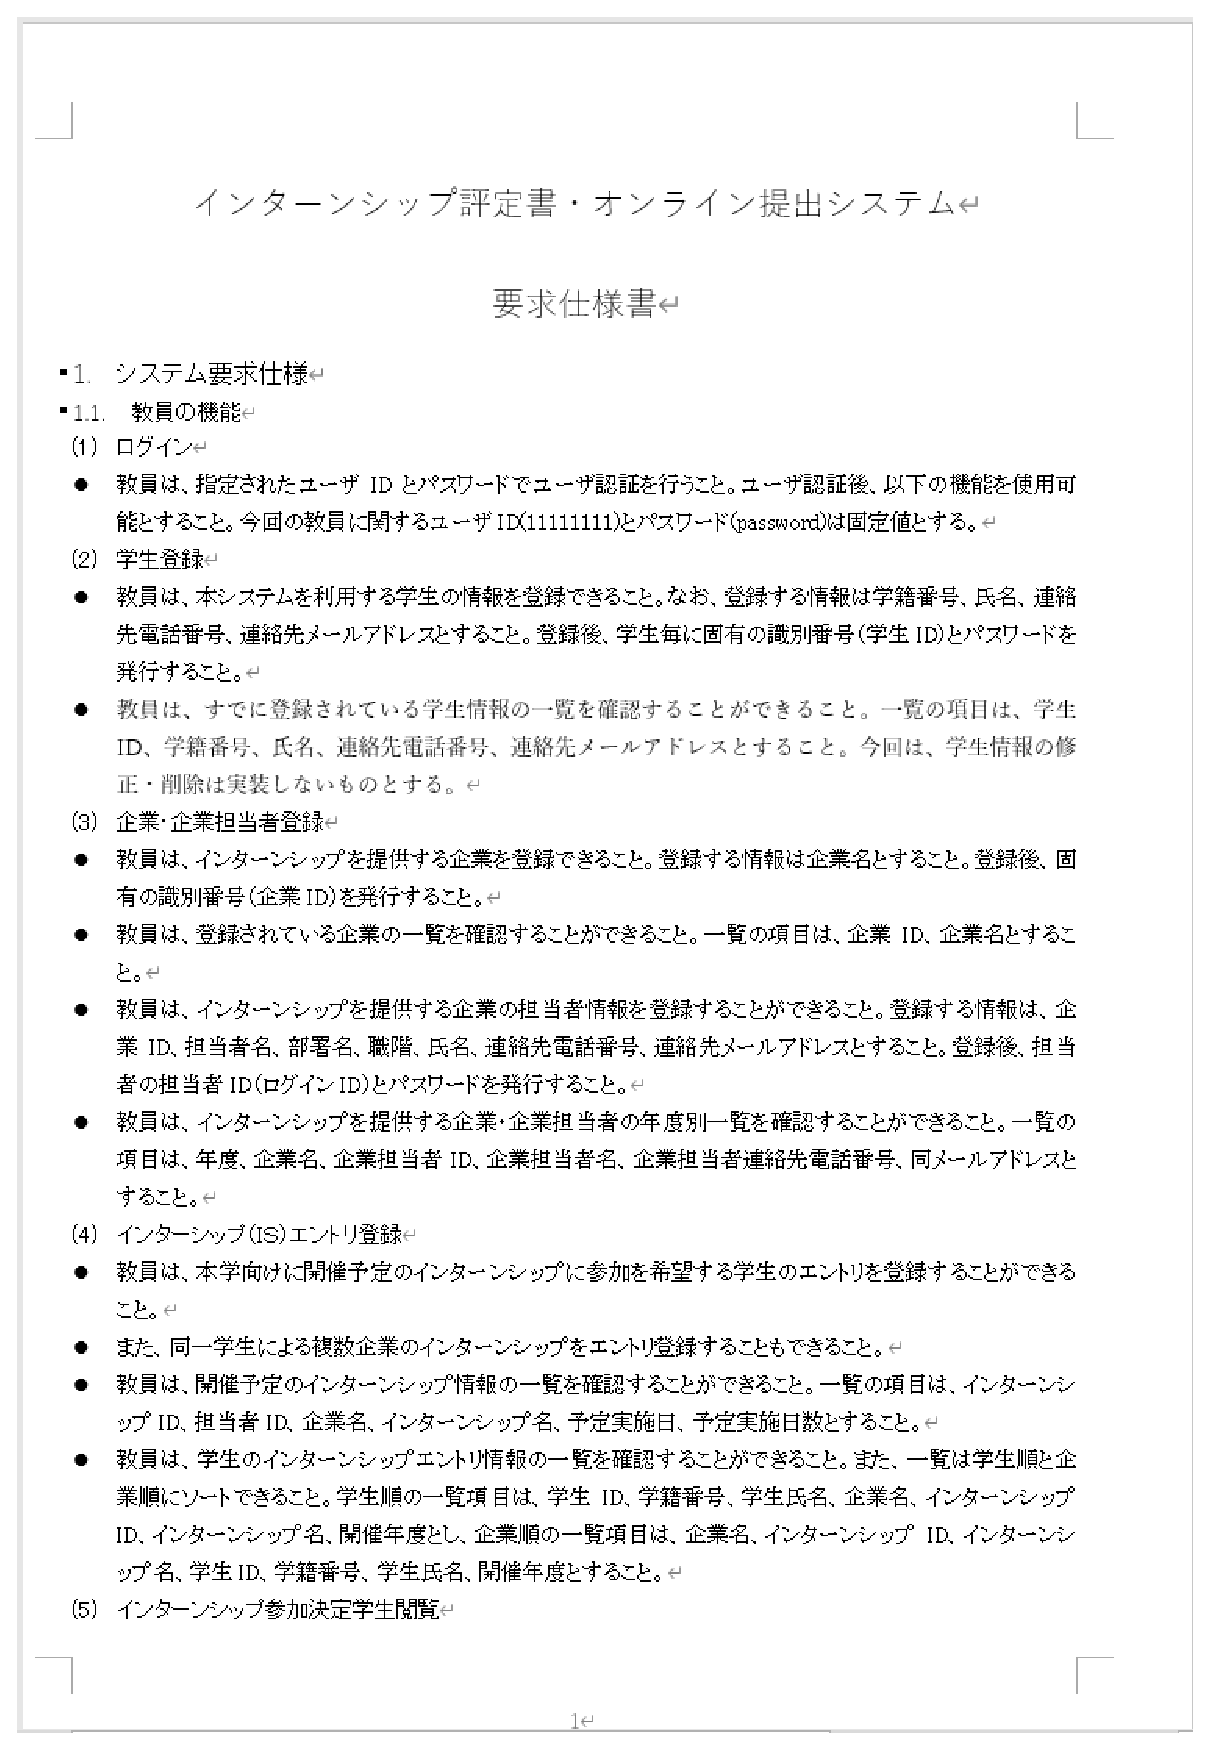
\includegraphics[width=\hsize]{specification/internship_1.eps}
    \end{center}
\end{figure}

\begin{figure}[tp]
    \begin{center}
    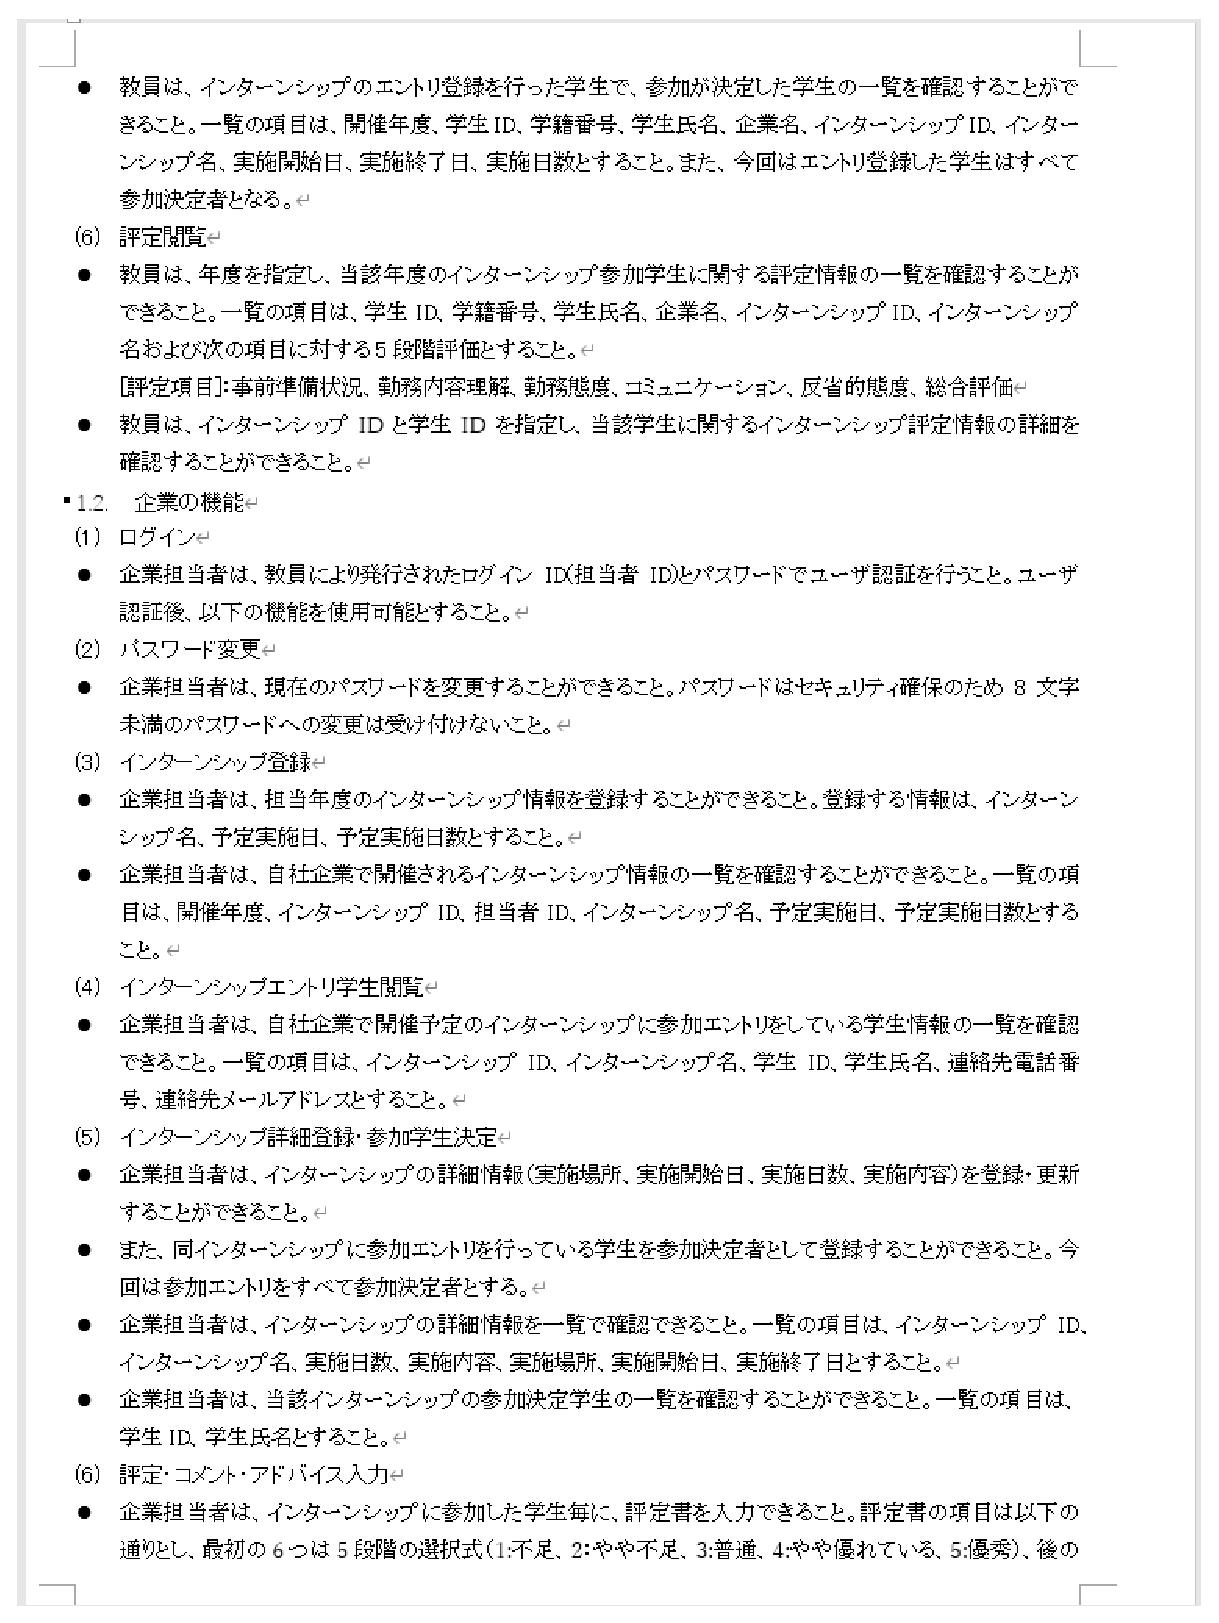
\includegraphics[width=\hsize]{specification/internship_2.eps}

    \end{center}
\end{figure}

\begin{figure}[tp]
    \begin{center}
    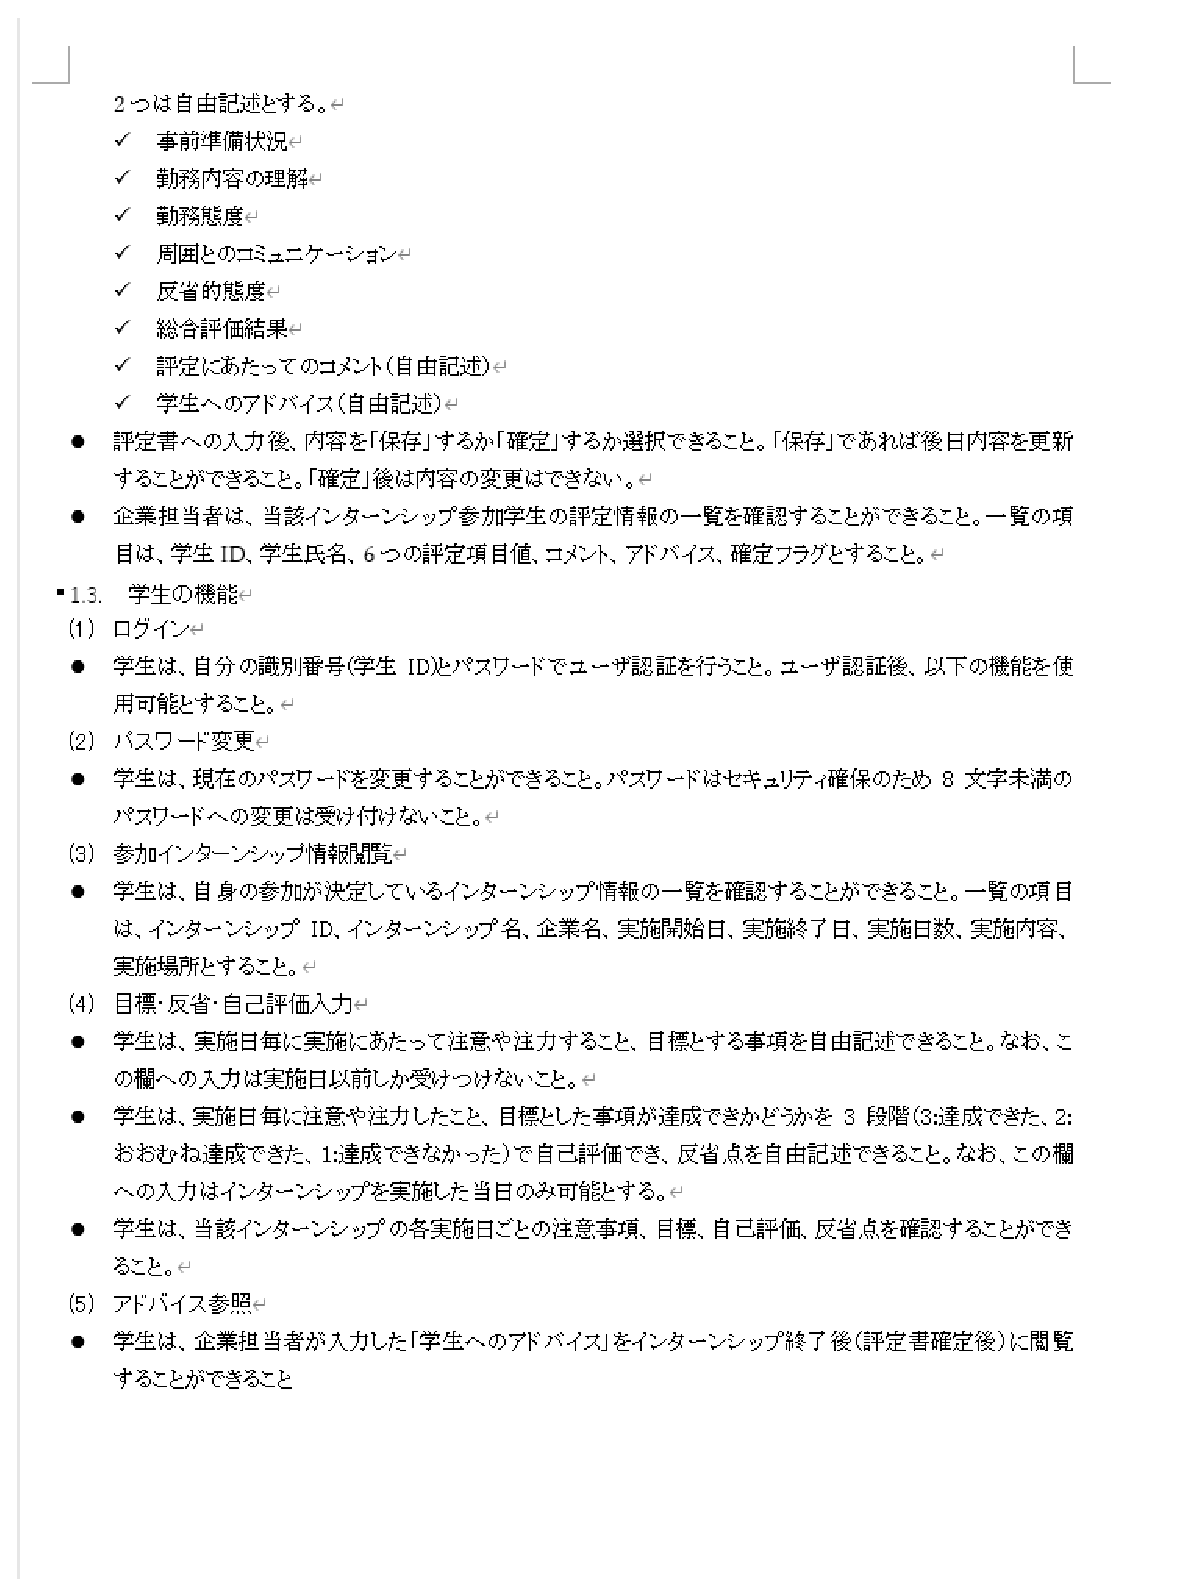
\includegraphics[width=\hsize]{specification/internship_3.eps}
    \end{center}
\end{figure}

\chapter{ETロボコン2020競技規約}    \label{ET_Specification}

\begin{figure}[tp]
    \begin{center}
    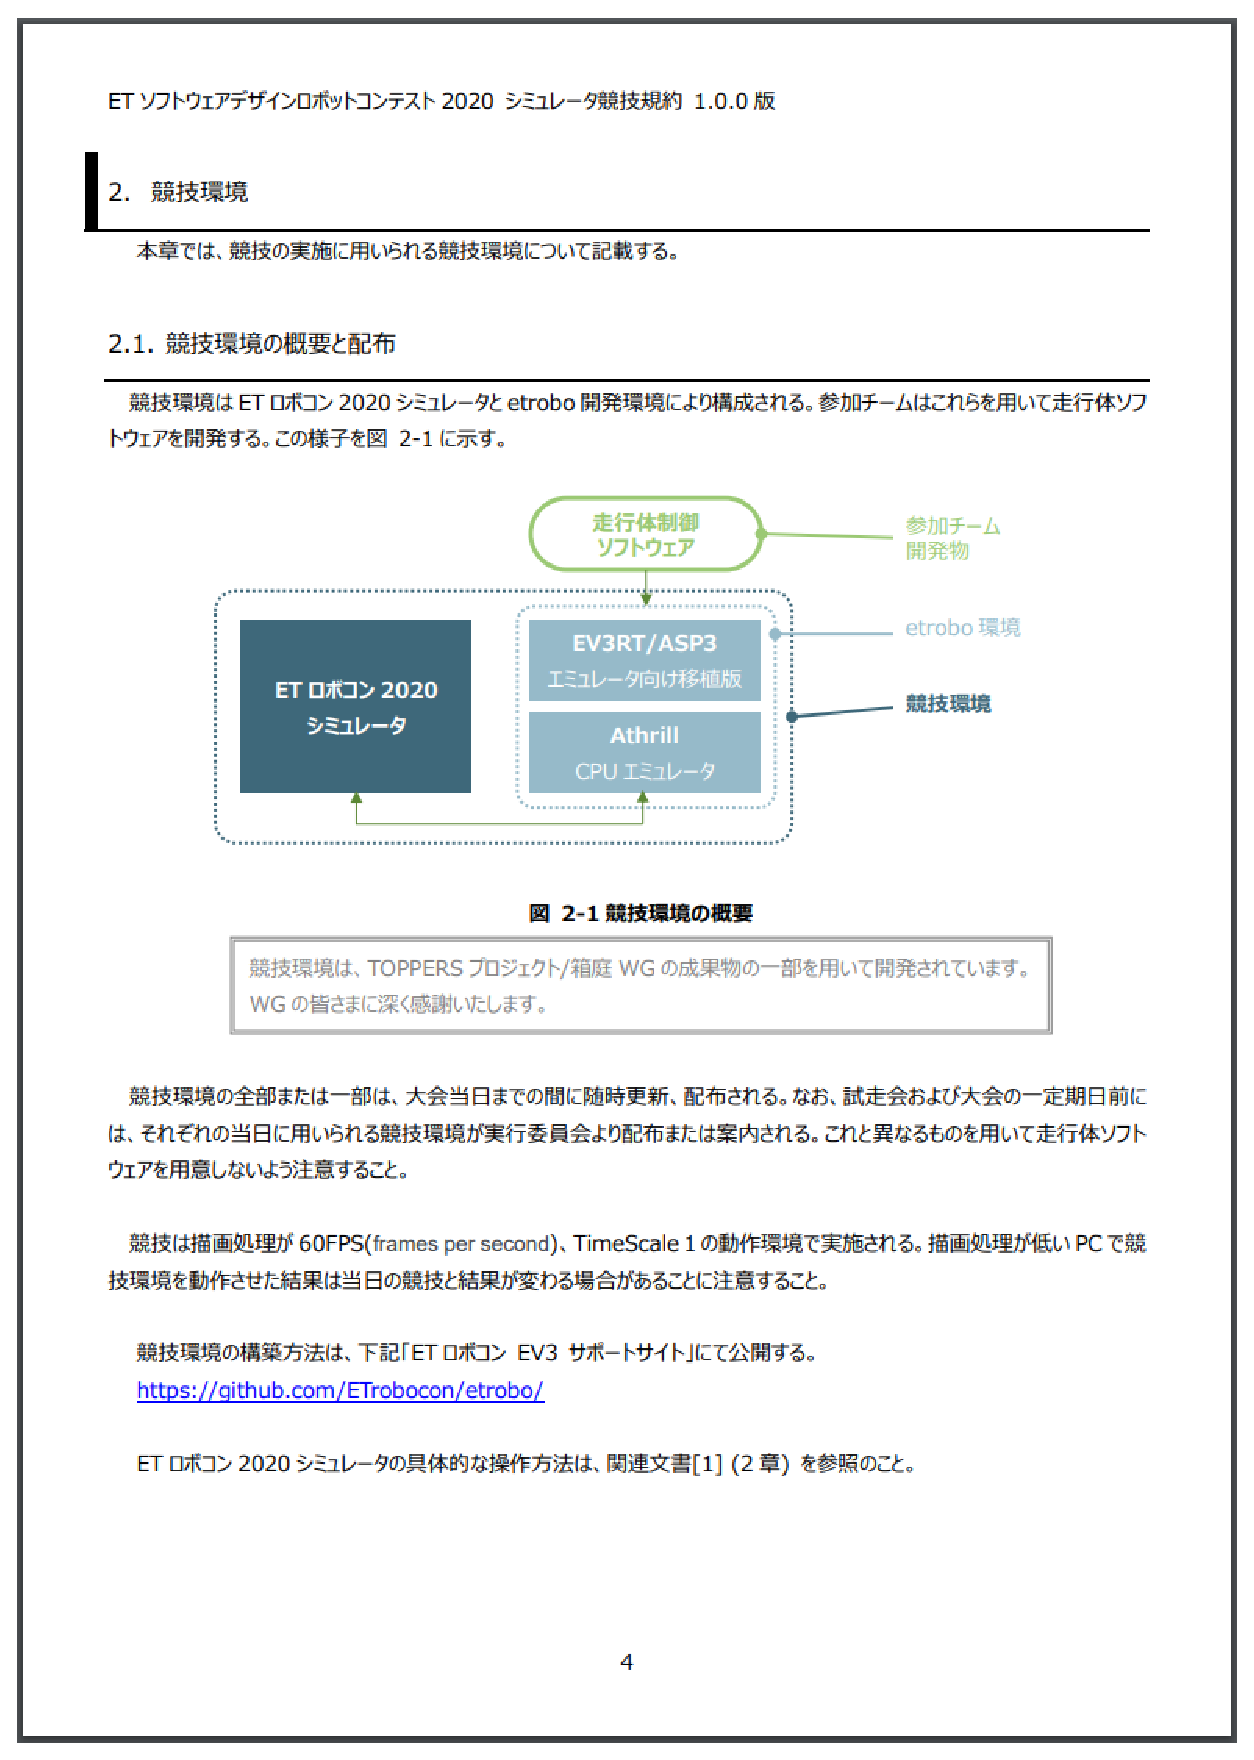
\includegraphics[width=\hsize]{specification/ET_1.eps}
    \end{center}
\end{figure}

\begin{figure}[tp]
    \begin{center}
    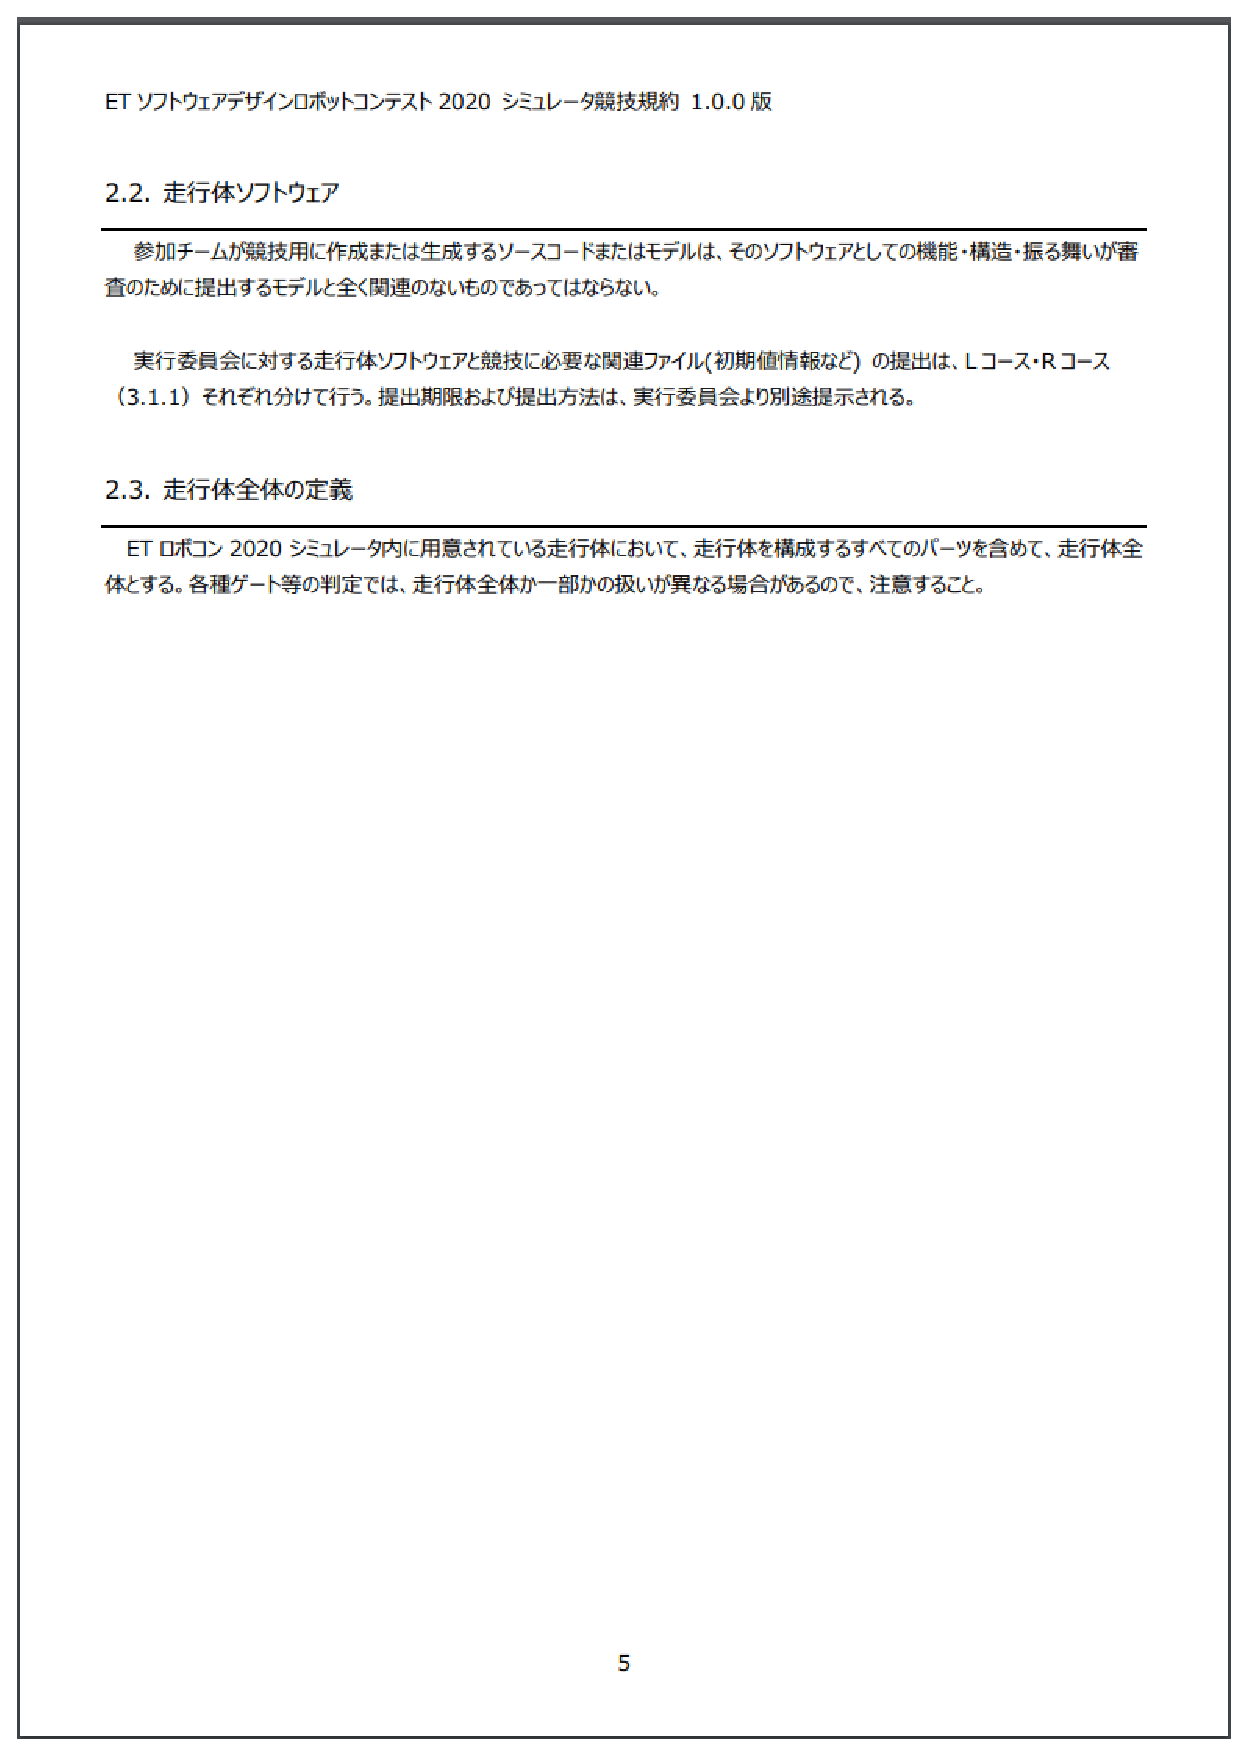
\includegraphics[width=\hsize]{specification/ET_2.eps}
    \end{center}
\end{figure}

\begin{figure}[tp]
    \begin{center}
    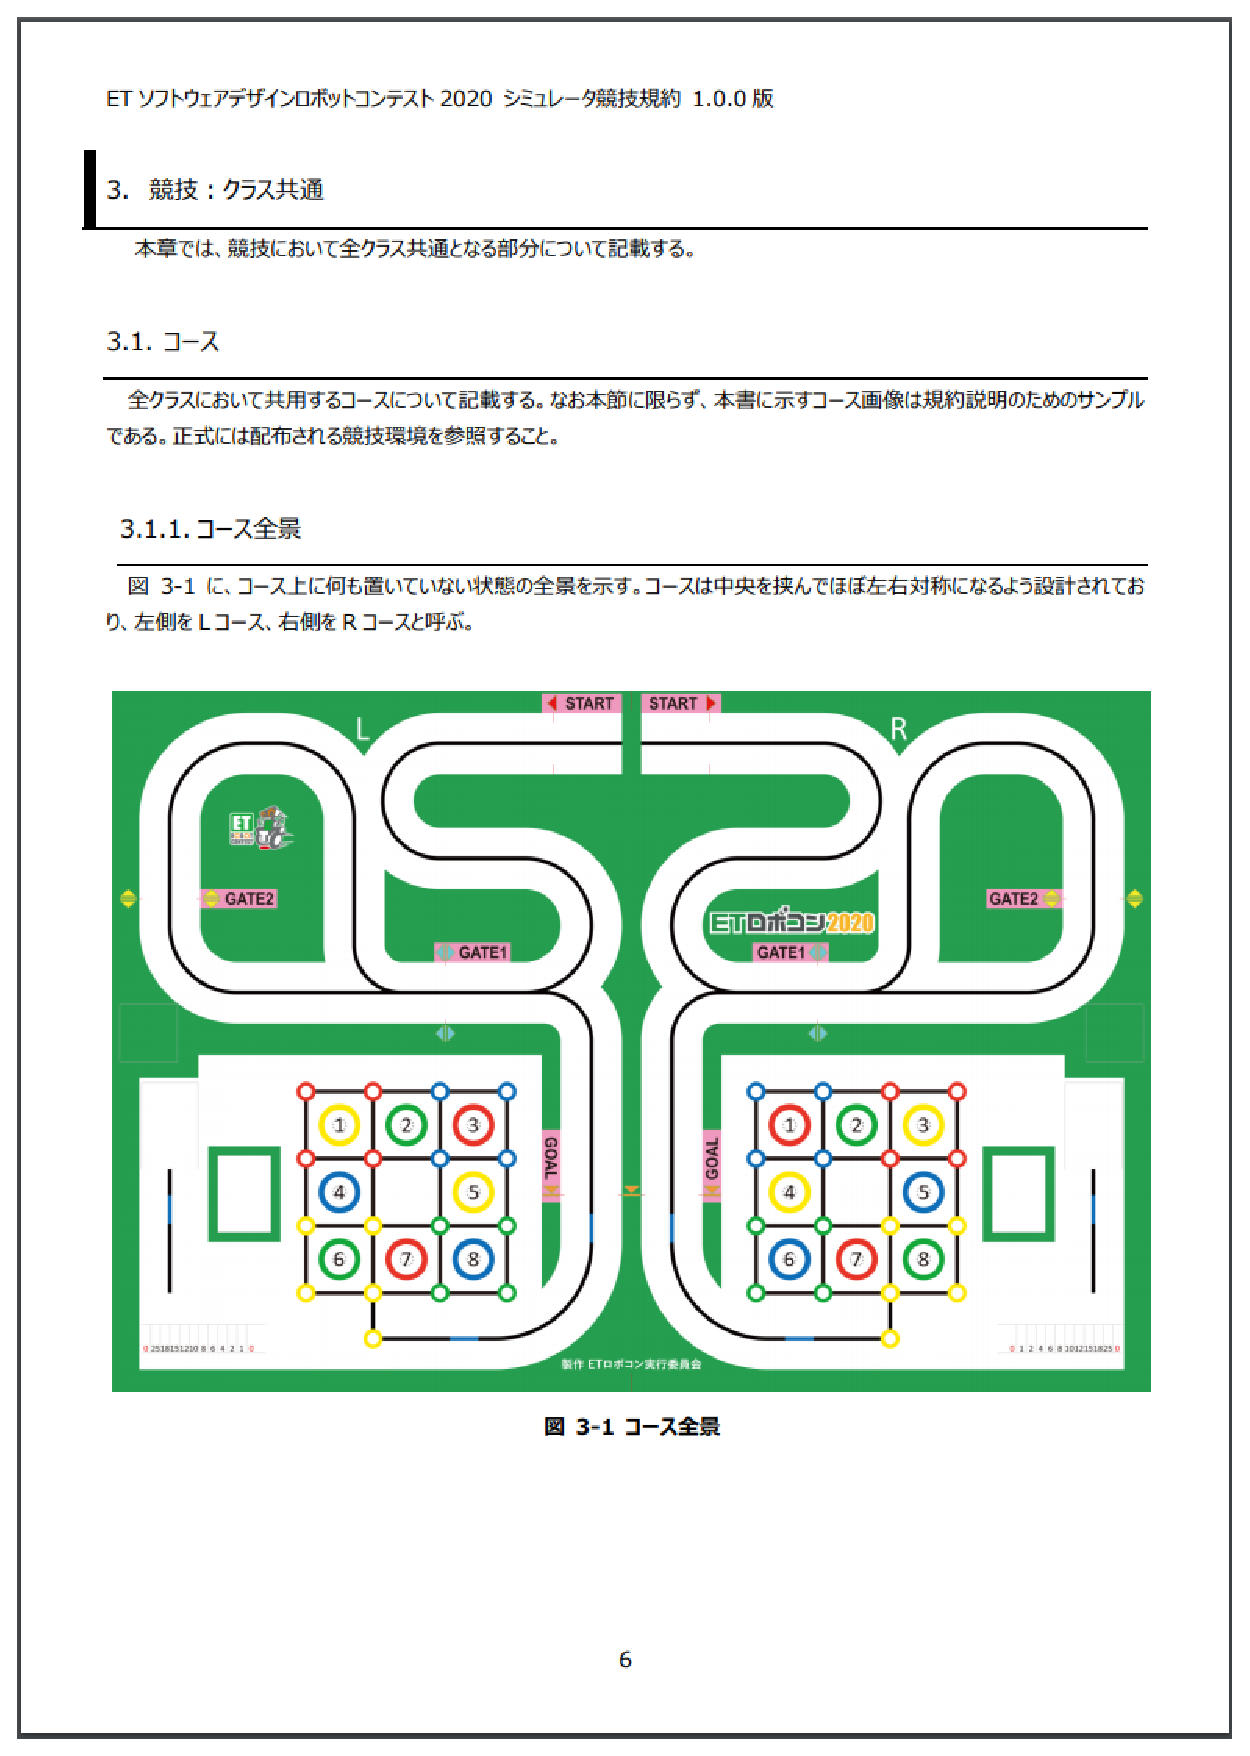
\includegraphics[width=\hsize]{specification/ET_3.eps}
    \end{center}
\end{figure}

\begin{figure}[tp]
    \begin{center}
    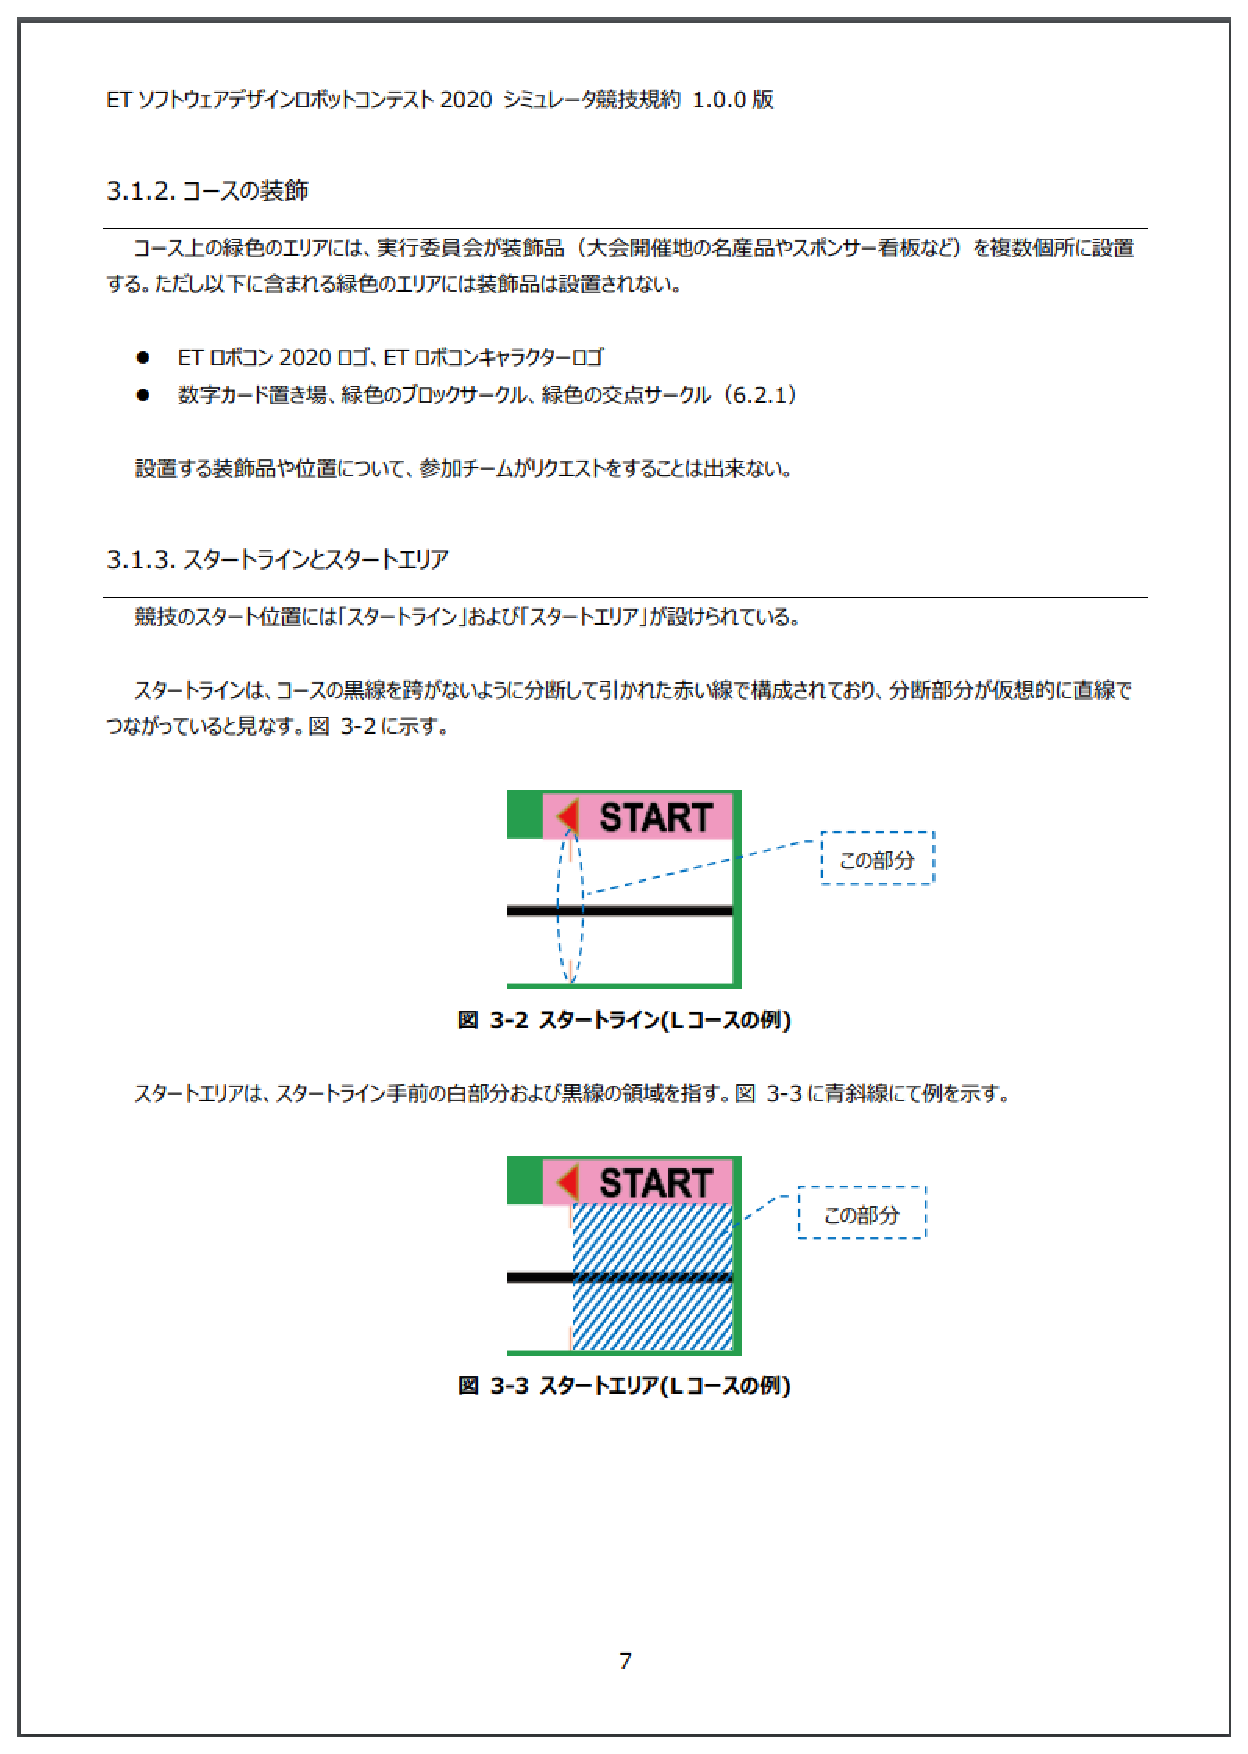
\includegraphics[width=\hsize]{specification/ET_4.eps}
    \end{center}
\end{figure}

\begin{figure}[tp]
    \begin{center}
    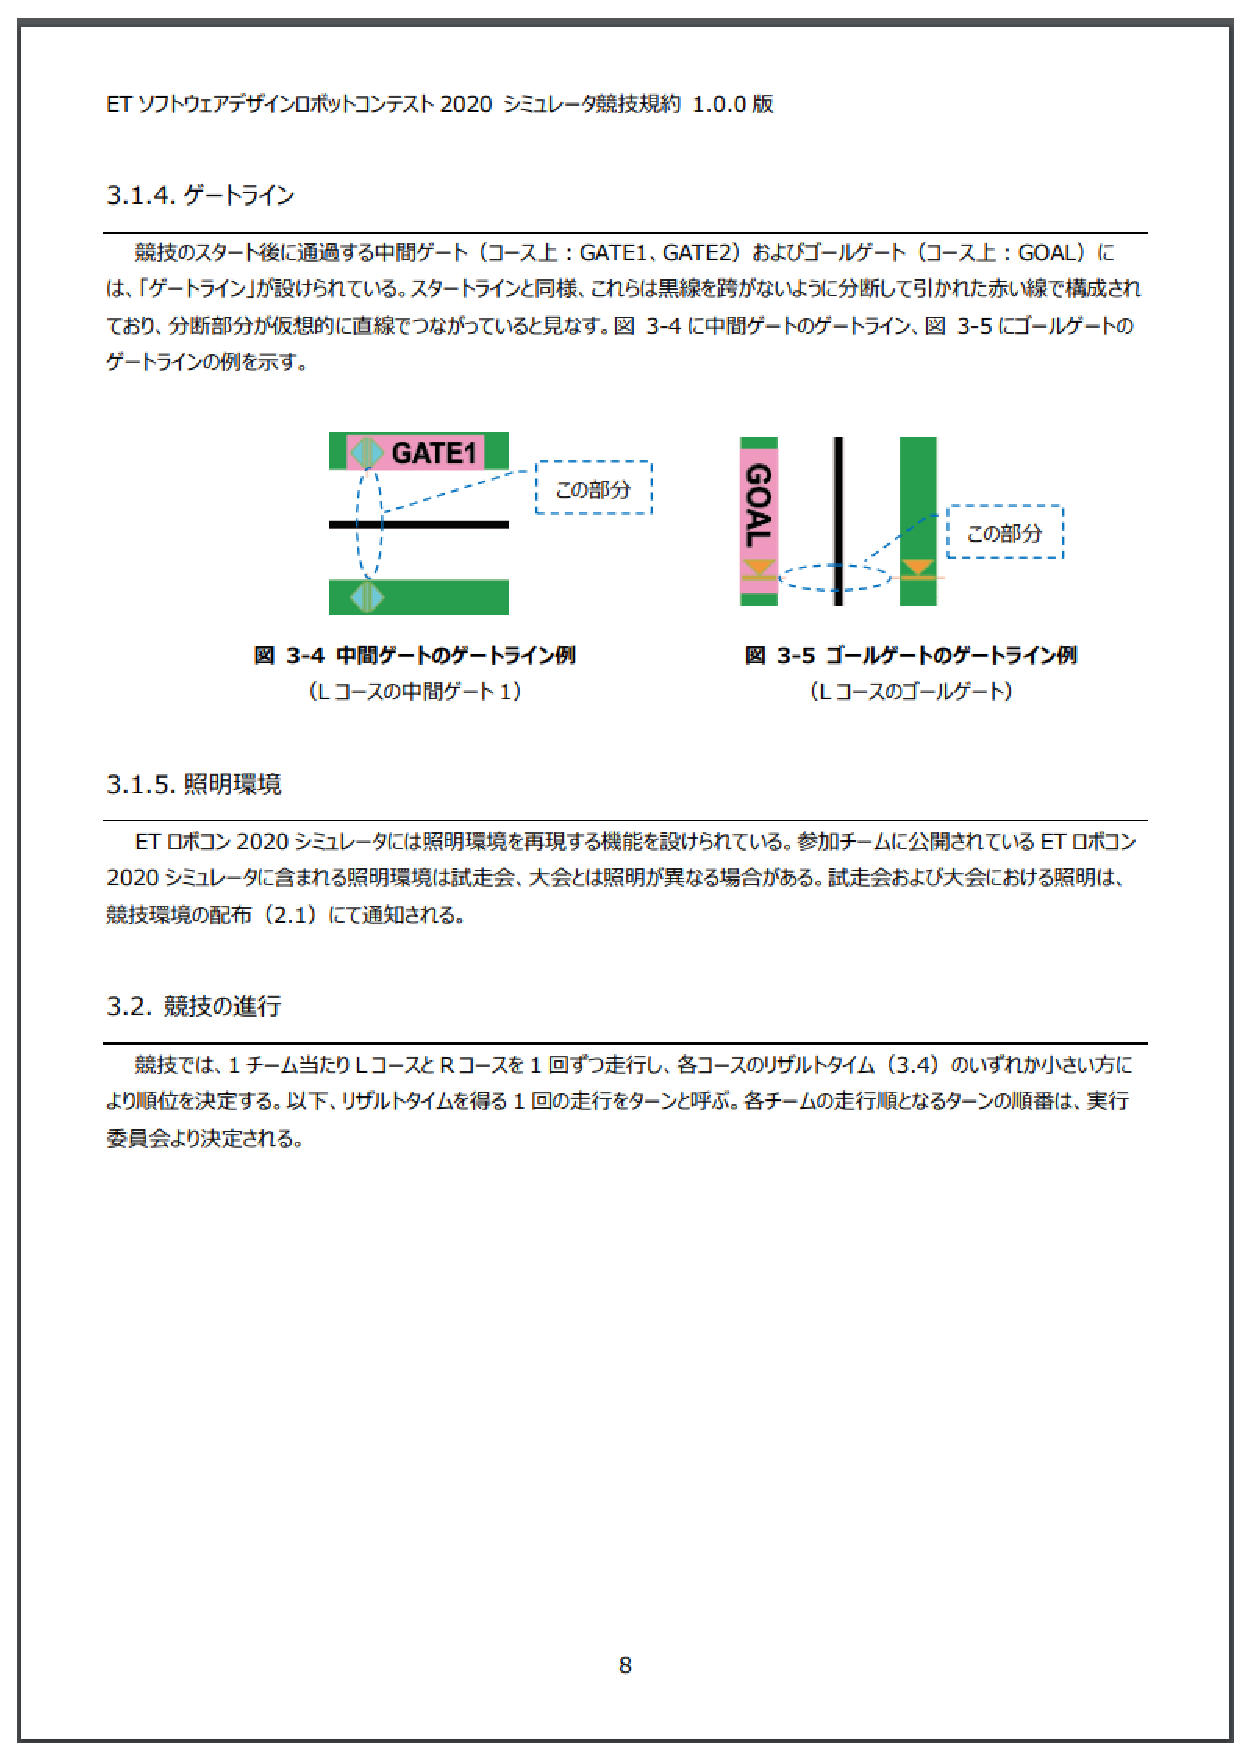
\includegraphics[width=\hsize]{specification/ET_5.eps}
    \end{center}
\end{figure}

\begin{figure}[tp]
    \begin{center}
    \includegraphics[width=\hsize]{specification/ET_6.eps}
    \end{center}
\end{figure}

\begin{figure}[tp]
    \begin{center}
    \includegraphics[width=\hsize]{specification/ET_7.eps}
    \end{center}
\end{figure}

\begin{figure}[tp]
    \begin{center}
    \includegraphics[width=\hsize]{specification/ET_8.eps}
    \end{center}
\end{figure}

\begin{figure}[tp]
    \begin{center}
    \includegraphics[width=\hsize]{specification/ET_9.eps}
    \end{center}
\end{figure}

\begin{figure}[tp]
    \begin{center}
    \includegraphics[width=\hsize]{specification/ET_10.eps}
    \end{center}
\end{figure}
\begin{figure}[tp]
    \begin{center}
    \includegraphics[width=\hsize]{specification/ET_11.eps}
    \end{center}
\end{figure}

\begin{figure}[tp]
    \begin{center}
    \includegraphics[width=\hsize]{specification/ET_12.eps}
    \end{center}
\end{figure}

\begin{figure}[tp]
    \begin{center}
    \includegraphics[width=\hsize]{specification/ET_13.eps}
    \end{center}
\end{figure}

\begin{figure}[tp]
    \begin{center}
    \includegraphics[width=\hsize]{specification/ET_14.eps}
    \end{center}
\end{figure}

\begin{figure}[tp]
    \begin{center}
    \includegraphics[width=\hsize]{specification/ET_15.eps}
    \end{center}
\end{figure}

\begin{figure}[tp]
    \begin{center}
    \includegraphics[width=\hsize]{specification/ET_16.eps}
    \end{center}
\end{figure}

\begin{figure}[tp]
    \begin{center}
    \includegraphics[width=\hsize]{specification/ET_17.eps}
    \end{center}
\end{figure}


% \newpage
% \listoftodos
\end{document}